\documentclass[12pt,reqno,oneside]{amsart}
\usepackage{import}
%===============================%
%  Packages and basic settings  %
%===============================%
\usepackage[headheight=15pt,rmargin=0.5in,lmargin=0.5in,tmargin=0.75in,bmargin=0.75in]{geometry}
\usepackage{imakeidx}
\usepackage{framed}
\usepackage{amssymb}
\usepackage{amsmath}
\usepackage{mathrsfs}
\usepackage{enumitem}
\usepackage{hyperref}
\usepackage{appendix}
\usepackage[capitalise,noabbrev]{cleveref}
\usepackage{tikz}
\usepackage{tikz-cd}
\usepackage{nomencl}\makenomenclature
\usetikzlibrary{braids,arrows,decorations.markings,calc}

%====================================%
%  Theorems, environments & cleveref  %
%====================================%
\newtheorem{theorem}{Theorem}[section]
\newtheorem{proposition}{Proposition}[section]
\newtheorem{corollary}{Corollary}[section]
\newtheorem{lemma}{Lemma}[section]
\newtheorem{conjecture}{Conjecture}[section]
\newtheorem{remark}{Remark}[section]

\newenvironment{stabular}[2][1]
  {\def\arraystretch{#1}\tabular{#2}}
  {\endtabular}

%==================================%
%  Custom commands & environments  %
%==================================%
\newcommand{\legendre}[2]{\left(\frac{#1}{#2}\right)}
\newcommand{\dlegendre}[2]{\displaystyle{\left(\frac{#1}{#2}\right)}}
\newcommand{\tlegendre}[2]{\textstyle{\left(\frac{#1}{#2}\right)}}
\newcommand{\psum}{\sideset{}{'}\sum}
\newcommand{\asum}{\sideset{}{^{\ast}}\sum}
\newcommand{\tmod}[1]{\ \left(\text{mod }#1\right)}
\newcommand{\xto}[1]{\xrightarrow{#1}}
\newcommand{\xfrom}[1]{\xleftarrow{#1}}
\newcommand{\normal}{\mathrel{\unlhd}}
\newcommand{\mf}{\mathfrak}
\newcommand{\mc}{\mathcal}
\newcommand{\ms}{\mathscr}

\newcommand{\Mat}{\mathrm{Mat}}
\newcommand{\GL}{\mathrm{GL}}
\newcommand{\SL}{\mathrm{SL}}
\newcommand{\PSL}{\mathrm{PSL}}
\renewcommand{\O}{\mathrm{O}}
\newcommand{\SO}{\mathrm{SO}}
\newcommand{\U}{\mathrm{U}}
\newcommand{\Sp}{\mathrm{Sp}}

\newcommand{\N}{\mathbb{N}}
\newcommand{\Z}{\mathbb{Z}}
\newcommand{\Q}{\mathbb{Q}}
\newcommand{\R}{\mathbb{R}}
\newcommand{\C}{\mathbb{C}}
\newcommand{\F}{\mathbb{F}}
\renewcommand{\H}{\mathbb{H}}
\renewcommand{\P}{\mathbb{P}}

\renewcommand{\a}{\alpha}
\renewcommand{\b}{\beta}
\newcommand{\g}{\gamma}
\renewcommand{\d}{\delta}
\newcommand{\z}{\zeta}
\renewcommand{\t}{\theta}
\renewcommand{\i}{\iota}
\renewcommand{\k}{\kappa}
\renewcommand{\l}{\lambda}
\newcommand{\s}{\sigma}
\newcommand{\w}{\omega}

\newcommand{\G}{\Gamma}
\newcommand{\D}{\Delta}
\renewcommand{\L}{\Lambda}
\newcommand{\W}{\Omega}

\newcommand{\e}{\varepsilon}
\newcommand{\vt}{\vartheta}
\newcommand{\vphi}{\varphi}
\newcommand{\emt}{\varnothing}

\newcommand{\x}{\times}
\newcommand{\ox}{\otimes}
\newcommand{\op}{\oplus}
\newcommand{\bigox}{\bigotimes}
\newcommand{\bigop}{\bigoplus}
\newcommand{\del}{\partial}
\newcommand{\<}{\langle}
\renewcommand{\>}{\rangle}
\newcommand{\lf}{\lfloor}
\newcommand{\rf}{\rfloor}
\newcommand{\wtilde}{\widetilde}
\newcommand{\what}{\widehat}
\newcommand{\conj}{\overline}
\newcommand{\cchi}{\conj{\chi}}

\DeclareMathOperator{\id}{\textrm{id}}
\DeclareMathOperator{\sgn}{\mathrm{sgn}}
\DeclareMathOperator{\im}{\mathrm{im}}
\DeclareMathOperator{\rk}{\mathrm{rk}}
\DeclareMathOperator{\tr}{\mathrm{trace}}
\DeclareMathOperator{\nm}{\mathrm{norm}}
\DeclareMathOperator{\ord}{\mathrm{ord}}
\DeclareMathOperator{\Hom}{\mathrm{Hom}}
\DeclareMathOperator{\End}{\mathrm{End}}
\DeclareMathOperator{\Aut}{\mathrm{Aut}}
\DeclareMathOperator{\Tor}{\mathrm{Tor}}
\DeclareMathOperator{\Ann}{\mathrm{Ann}}
\DeclareMathOperator{\Gal}{\mathrm{Gal}}
\DeclareMathOperator{\Trace}{\mathrm{Trace}}
\DeclareMathOperator{\Norm}{\mathrm{Norm}}
\DeclareMathOperator{\Span}{\mathrm{Span}}
\DeclareMathOperator*{\Res}{\mathrm{Res}}
\DeclareMathOperator{\Vol}{\mathrm{Vol}}
\DeclareMathOperator{\Li}{\mathrm{Li}}
\renewcommand{\Re}{\mathrm{Re}}
\renewcommand{\Im}{\mathrm{Im}}

\newcommand{\GH}{\G\backslash\H}
\newcommand{\GG}{\G_{\infty}\backslash\G}

\newenvironment{psmallmatrix}
  {\left(\begin{smallmatrix}}
  {\end{smallmatrix}\right)}

%============%
%  Comments  %
%============%
\newcommand{\todo}[1]{\textcolor{red}{\sf Todo: [#1]}}

%===================%
%  Label reminders  %
%===================%
% [label=(\roman*)]
% [label=(\alph*)]
% [label=(\arabic{enumi})]

%==================%
%  Other settings  %
%==================%
\pgfdeclarelayer{background}
\pgfsetlayers{background,main}
\tikzset{->-/.style={decoration={
  markings,
  mark=at position .5 with {\arrow{>}}},postaction={decorate}}}

%=================%
%  Title & Index  %
%=================%
\title{A quadratic double Dirichlet series I: the function field case}
\author{Henry Twiss}
\date{2024}
\makeindex

\begin{document}

\begin{abstract}
    We construct a quadratic double Dirichlet series $Z(s,w)$ built from single variable quadratic Dirichlet $L$-functions $L(s,\chi)$ attached to the functional field $\F_{q}(t)$. We prove that $Z(s,w)$ admits meromorphic continuation to the $(s,w)$-plane and satisfies a group of functional equations. We also outline an application of the usefulness of $Z(s,w)$ and show that it is a rational function in $x = q^{-s}$ and $y = q^{-w}$. This is the simplest construction of a quadratic Weyl group multiple Dirichlet series over a global field.
\end{abstract}

\maketitle

\section{Preliminaries}
    We will give an overview of the zeta function and quadratic Dirichlet $L$-functions attached to $\F_{q}(t)$. For proofs of these facts and a more detailed analysis see \cite{rosen2002number}. Let $q$ be a power of an odd prime and let $\F_{q}[t]$ be the polynomial ring in $t$ with coefficients in the finite field $\F_{q}$. This is a principal ideal domain. Moreover, the nonzero prime ideals in $\F_{q}[t]$ are generated by irreducible polynomials. Let $\F_{q}(t)$ denote the quotient field. Define the norm function $N(m)$ by
    \[
        N(m) = |m| = q^{\deg(m)},
    \]
    for any $m \in \F_{q}[t]$. The zeta function $\z(s)$ on $\F_{q}[t]$ is defined as the Dirichlet series or Euler product
    \[
        \z(s) = \sum_{\text{$m$ monic}}\frac{1}{|m|^{s}} = \prod_{\text{$P$ monic irr}}\left(1-\frac{1}{|P|^{s}}\right)^{-1},
    \]
    where the second equality holds since $\F_{q}[t]$ is a unique factorization domain. As for questions of convergence, there are $q^{n}$ monic polynomials of degree $n$ so, provided $\Re(s) > 1$, we can sum up the Dirichlet series according to degree and obtain an explicit expression:
    \[
        \z(s) = \sum_{n \ge 0}\frac{\text{\# of monic poly of deg $n$}}{q^{ns}} = \sum_{n \ge 1}\frac{1}{q^{n(1-s)}} = \frac{1}{1-q^{1-s}}.
    \]
    The latter expression is meromorphic on $\C$ with a simple pole at $s = 1$ of residue $\frac{1}{\log(q)}$. Therefore $\z(s)$ admits meromorphic continuation to $\C$. The zeta function also satisfies a functional equation. Define the completed zeta function $\z^{\ast}(s)$ (this is also the zeta function attached to $\F_{q}(t)$) by
    \[
        \z^{\ast}(s) = \frac{1}{1-q^{-s}}\z(s).
    \]
    Then
    \[
        \z^{\ast}(s) = q^{2s-1}\z^{\ast}(1-s).
    \]
    Recall that characters on $\F_{q}[t]$ are multiplicative functions $\chi:\F_{q}[t] \to \C$. They form a group under multiplication. The two flavors we will care about are:
    
    \begin{itemize}
        \item Dirichlet characters: multiplicative functions $\chi_{d}:\F_{q}[t] \to \C$ modulo $d \in \F_{q}[t]$ (in that they are $d$-periodic) and such that $\chi_{d}(m) = 0$ if $(m,d) > 1$.
        \item Hilbert characters: The group of characters generated by those that appear in the sign change of reciprocity statements.
    \end{itemize}
    
    The image of a Dirichlet character always lands in the roots of unity. Moreover, $\conj{\chi}$ is the multiplicative inverse to $\chi$ and the Dirichlet characters modulo $d$ form a subgroup under multiplication. This group is always finite and its order is $\vphi(d) = |(\F_{q}[t]/d\F_{q}[t])^{\x}|$. The Dirichlet characters that are of interest to us are those attached to quadratic extensions of $\F_{q}[t]$ which, in turn, arise from the quadratic residue symbol. First let us recall this symbol. For any irreducible $p \in \F_{q}[t]$ and any $d \in \F_{q}[t]$, we define the quadratic residue symbol $\tlegendre{d}{p}$ by
    \[
        \legendre{d}{p} \equiv d^{\frac{|p|-1}{2}} \tmod{p} = \begin{cases} 1 & \text{if $x^{2} \equiv d \tmod{p}$ is solvable}, \\ -1 & \text{if $x^{2} \equiv d \tmod{p}$ is not solvable}, \\ 0 & \text{if $d \equiv 0 \tmod{p}$}. \end{cases}
    \]
    This symbol is only dependent upon $d$ modulo $p$ and is multiplicative in $d$. Moreover, if $b \in \F_{q}^{\ast}$, we have
    \[
        \legendre{b}{p} = \sgn(b)^{\deg(p)}.
    \]
    where $\sgn(b) = \pm1$ depending on if $b \in (\F_{q}^{\x})^{2}$ or not. Moreover, for $d \in \F_{q}[t]$ we have $\sgn(d) = \sgn(b_{n})$ if $d(t) = b_{n}t^{n}+b_{n-1}t^{n+1}+\cdots+b_{0}$ (with $b_{n} \neq 0$). We can extend the quadratic residue symbol multiplicatively in the denominator. If $m = bp_{1}^{e_{1}}p_{2}^{e_{2}} \cdots p_{k}^{e_{k}}$ is the prime factorization of $m$ (with $b \in \F_{q}^{\ast}$), then we define
    \[
        \legendre{d}{m} = \prod_{1 \le i \le k}\legendre{d}{p_{i}}^{e_{i}}.
    \]
    So the quadratic residue symbol now makes sense for any nonzero $m \in \F_{q}[t]$. Moreover, it only depends upon $d$ modulo $m$, the ideal generated by $m$, and is multiplicative in $m$. The quadratic residue symbol also admits the following reciprocity law:

    \begin{theorem}[Quadratic reciprocity]
        If $d,m \in \F_{q}[t]$ are nonzero with $(d,m) = 1$, then
        \[
            \legendre{d}{m} = (-1)^{\frac{q-1}{2}\deg(d)\deg(m)}\sgn(d)^{\deg(m)}\sgn(m)^{-\deg(d)}\legendre{m}{d}.
        \]
    \end{theorem}

    Note that if $q \equiv 1 \tmod{4}$ and $d$ and $m$ are monic, then the sign in the statement of quadratic reciprocity is always $1$ so that reciprocity is perfect:
    \[
        \legendre{d}{m} = \legendre{m}{d}.
    \]
    We can now define the quadratic Dirichlet characters. For any nonzero square-free monic $d \in \F_{q}[t]$, define the quadratic Dirichlet character $\chi_{d}$ by the following quadratic residue symbol:
    \[
        \chi_{d}(m) = \legendre{d}{m}.
    \]
    This quadratic Dirichlet character is attached to the quadratic extension $\F_{q}(t)(\sqrt{d})$. If $b \in \F_{q}^{\x}$, we define $\chi_{b}$ by
    \[
        \chi_{b}(m) = \legendre{b}{m} = \sgn(b)^{\deg(m)}.
    \]
    We extend $\chi_{d}$ multiplicatively in the denominator so that $\chi_{d}$ makes sense for any nonzero $d \in \F_{q}[t]$. In particular, $\chi_{d}(m) = \pm1$ provided $d$ and $m$ are relatively prime and $\chi_{d}(m) = 0$ if $(m,d) > 1$. Quadratic reciprocity implies that $\chi_{d}$ is a Dirichlet character modulo $d$. Indeed, for any $m$ we can take $d$ modulo $m$ so that $\deg(d+m) = \deg(m)$ and $\sgn(d+m) = \sgn(m)$. Lastly, note that if $q \equiv 1 \tmod{4}$ and $d$ and $m$ are monic, then
    \[
        \chi_{d}(m) = \chi_{m}(d),
    \]
    which is a reformulation of reciprocity being perfect. We now discuss the Hilbert characters. We will only need two of them: one nontrivial and one trivial. The nontrivial Hilbert character is $\chi_{\t}$ where $\t \in \F^{\x}-(\F^{\x})^{2}$:
    \[
        \chi_{\t}(m) = (-1)^{\deg(m)}.
    \]
    Note that $\conj{\chi_{\t}} = \chi_{\t}$. The other Hilbert character is the trivial Dirichlet character $\chi_{\t}^{2} = \chi_{\t\t} = \chi_{1}$. In general, we denote a Hilbert character by $\chi_{a}$ where $a \in \{1,\t\}$. The Hilbert characters also satisfy an important orthogonality property:

    \begin{theorem}[Orthogonality of Hilbert characters]
        If $d,m \in \F_{q}[t]$ are nonzero, then
        \[
            \frac{1}{2}\sum_{a \in \{1,\t\}}\chi_{a}(dm) = \begin{cases} 1 & \text{if $\deg(d) \equiv \deg(m) \tmod{2}$}, \\ 0 & \text{if $\deg(d) \not\equiv \deg(m) \tmod{2}$}. \end{cases}
        \]
    \end{theorem}
    
    More generally, we would also require Hilbert characters to keep track of the $(-1)^{\frac{q-1}{2}\deg(d)\deg(m)}$ factor in the statement of quadratic reciprocity but as we will assume $q \equiv 1 \tmod{4}$, we will not require this additional difficulty. With the Dirichlet and Hilbert characters introduced, we are ready to discuss the $L$-functions associated to quadratic Dirichlet characters. We define the Dirichlet $L$-function $L(s,\chi_{d})$ attached to $\chi_{d}$ for square-free $d$, by a Dirichlet series or Euler product:
    \[
        L(s,\chi_{d}) = \sum_{\text{$m$ monic}}\frac{\chi_{d}(m)}{|m|^{s}} = \prod_{\text{$P$ monic irr}}\left(1-\frac{\chi_{d}(P)}{|P|^{s}}\right)^{-1}.
    \]
    By definition of the quadratic Dirichlet character, $L(s,\chi_{d}) \ll \z(s)$ for $\Re(s) > 1$ so that $L(s,\chi_{d})$ is locally absolutely uniformly convergent in this region. $L(s,\chi_{d})$ also admits analytic continuation to $\C$ (see \cite{rosen2002number} for a proof). Moreover, $L(s,\chi_{d})$ is a polynomial in $q^{-s}$ of degree at most $\deg(d)-1$. The associated completed Dirichlet $L$-function $L^{\ast}(s,\chi_{d})$ is defined as
    \[
        L^{\ast}(s,\chi_{d}) = \begin{cases} \frac{1}{1-q^{-s}}L(s,\chi_{d}) & \text{if $\deg(d)$ is even}, \\ L(s,\chi_{d}) & \text{if $\deg(d)$ is odd}, \end{cases}
    \]
    and satisfies the functional equation
    \[
        L^{\ast}(s,\chi_{d}) = \begin{cases} q^{2s-1}|d|^{\frac{1}{2}-s}L^{\ast}(1-s,\chi_{d}) & \text{if $\deg(d)$ is even}, \\ q^{2s-1}(q|d|)^{\frac{1}{2}-s}L^{\ast}(1-s,\chi_{d}) & \text{if $\deg(d)$ is odd}. \end{cases}
    \]
    Note that in the case $\deg(d)$ is even, the conductor is $|d|$ and in the case $\deg(d)$ is odd, the conductor is $q|d|$. Moreover, the gamma factors depend upon the degree of $d$. This will cause a small but important technical issue later when we want to derive functional equations for the quadratic double Dirichlet series. Analogously (this is a superfluous definition but we are giving it to be consistent with notation for the quadratic double Dirichlet series later on), we define the Dirichlet $L$-function $L(w,\chi_{m})$ attached to $\chi_{m}$ for square-free $m$, by a Dirichlet series or Euler product:
    \[
        L(w,\chi_{m}) = \sum_{\text{$d$ monic}}\frac{\chi_{m}(d)}{|d|^{w}} = \prod_{\text{$P$ monic irr}}\left(1-\frac{\chi_{m}(P)}{|P|^{w}}\right)^{-1}.
    \]
    As for $L(s,\chi_{d})$, $L(w,\chi_{m}) \ll \z(w)$ for $\Re(w) > 1$ so that $L(w,\chi_{m})$ is locally absolutely uniformly convergent in this region. Moreover, $L(w,\chi_{m})$ admits analytic continuation to $\C$ and is a polynomial in $q^{-w}$ of degree at most $\deg(m)-1$. The associated completed Dirichlet $L$-function $L^{\ast}(w,\chi_{m})$ is defined as
    \[
        L^{\ast}(w,\chi_{m}) = \begin{cases} \frac{1}{1-q^{-w}}L(w,\chi_{m}) & \text{if $\deg(m)$ is even}, \\ L(w,\chi_{m}) & \text{if $\deg(m)$ is odd}, \end{cases}
    \]
    and satisfies the functional equation
    \[
        L^{\ast}(w,\chi_{m}) = \begin{cases} q^{2w-1}|d|^{\frac{1}{2}-w}L^{\ast}(1-w,\chi_{m}) & \text{if $\deg(m)$ is even}, \\ q^{2w-1}(q|m|)^{\frac{1}{2}-w}L^{\ast}(1-w,\chi_{m}) & \text{if $\deg(m)$ is odd}. \end{cases}
    \]

    \begin{remark}
        The definitions for $L(s,\chi_{d})$, $L^{\ast}(s,\chi_{d})$, $L(w,\chi_{m})$, and $L^{\ast}(w,\chi_{m})$ hold even when $d$ and $m$ are not square-free (however the functional equations do not hold). We will make use of slightly modified definitions in this case and so we purposely do not define these $L$-functions yet.
    \end{remark}
\section{The Quadratic Double Dirichlet Series}
    From now on we assume $q \equiv 1 \tmod{4}$. This assumption is not strictly necessary to build the quadratic double Dirichlet series but it does allow for some technical simplifications as the statement of quadratic reciprocity is perfect. We are ready to define the quadratic double Dirichlet series $Z(s,w)$. For any monic $d \in \F_{q}[t]$, write $d = d_{0}d_{1}^{2}$ where $d_{0}$ is square-free. In other words, $d_{0}$ is the square-free part of $d$ so that $\frac{d}{d_{0}}$ is a perfect square. The \textbf{quadratic double Dirichlet series} $Z(s,w)$ is defined as
    \[
        Z(s,w) = \sum_{\text{$d$ monic}}\frac{L(s,\chi_{d_{0}})Q_{d_{0}d_{1}^{2}}(s)}{|d|^{w}},
    \]
    where $Q_{d_{0}d_{1}^{2}}(s)$ is the \textbf{correction polynomial} defined by
    \[
        Q_{d_{0}d_{1}^{2}}(s) = \sum_{e_{1}e_{2} \mid d_{1}}\mu(e_{1})\chi_{d_{0}}(e_{1})|e_{1}|^{-s}|e_{2}|^{1-2s} = \sum_{e_{1}e_{2}e_{3} = d_{1}}\mu(e_{1})\chi_{d_{0}}(e_{1})|e_{1}|^{-s}|e_{2}|^{1-2s},
    \]
    and $\mu$ is the usual M\"obius function on $\F_{q}[t]$. For $\Re(s) > 1$, we have the trivial bound
    \[
        Q_{d_{0}d_{1}^{2}}(s) \ll \sum_{e_{1}e_{2} \mid d_{1}}1 \ll \s_{0}(d_{1})^{2} \ll_{\e} |d|^{\e},
    \]
    for any $\e > 0$. Combining this estimate with the bound $L(s,\chi_{d_{0}}) \ll 1$ for $\Re(s) > 1$, we see that $Z(s,w)$ is locally absolutely uniformly convergent in the region $\L = \{(s,w) \in \C^{2}:\Re(s) > 1, \Re(w) > 1\}$. While $Z(s,w)$ is the double Dirichlet series we are after, it will be necessary to consider quadratic double Dirichlet series twisted by a pair of Hilbert characters $\chi_{a_{1}}$ and $\chi_{a_{2}}$. The \textbf{quadratic double Dirichlet series} $Z_{a_{1},a_{2}}(s,w)$ twisted by $\chi_{a_{1}}$ and $\chi_{a_{2}}$ is defined as
    \[
        Z_{a_{1},a_{2}}(s,w) = \sum_{\text{$d$ monic}}\frac{L(s,\chi_{a_{1}d_{0}})\chi_{a_{2}}(d)Q_{d_{0}d_{1}^{2}}(s,\chi_{a_{1}})}{|d|^{w}},
    \]
    where $Q_{d_{0}d_{1}^{2}}(s,\chi_{a_{1}})$ is the \textbf{correction polynomial} twisted by $\chi_{a_{1}}$ defined by
    \[
        Q_{d_{0}d_{1}^{2}}(s,\chi_{a_{1}}) = \sum_{e_{1}e_{2} \mid d_{1}}\mu(e_{1})\chi_{a_{1}d_{0}}(e_{1})|e_{1}|^{-s}|e_{2}|^{1-2s} = \sum_{e_{1}e_{2}e_{3} = d_{1}}\mu(e_{1})\chi_{a_{1}d_{0}}(e_{1})|e_{1}|^{-s}|e_{2}|^{1-2s},
    \]
    and $\mu$ is the usual M\"obius function on $\F_{q}[t]$. As the Hilbert characters are given by quadratic Dirichlet characters, we have the analogous bound $Q_{d_{0}d_{1}^{2}}(s,\chi_{a_{1}}) \ll |d|_{\e}$ so that $Z_{a_{1},a_{2}}(s,w)$ converges locally absolutely uniformly in the same region as $Z(s,w)$ does. In this generalized setup, $Z(s,w) = Z_{1,1}(s,w)$. Analogously, writing $m = m_{0}m_{1}^{2}$, the \textbf{quadratic double Dirichlet series} $Z(w,s)$ is defined as
    \[
        Z(w,s) = \sum_{\text{$m$ monic}}\frac{L(w,\chi_{m_{0}})Q_{m_{0}m_{1}^{2}}(w)}{|m|^{s}},
    \]
    where $Q_{m_{0}m_{1}^{2}}(w)$ is the \textbf{correction polynomial} defined by
    \[
        Q_{m_{0}m_{1}^{2}}(w) = \sum_{e_{1}e_{2} \mid m_{1}}\mu(e_{1})\chi_{m_{0}}(e_{1})|e_{1}|^{-w}|e_{2}|^{1-w} = \sum_{e_{1}e_{2}e_{3} = m_{1}}\mu(e_{1})\chi_{m_{0}}(e_{1})|e_{1}|^{-w}|e_{2}|^{1-w},
    \]
    and $\mu$ is the usual M\"obius function. We have the analogous estimate $Q_{m_{0}m_{1}^{2}}(w) \ll_{\e} |m|^{\e}$ and since $L(w,\chi_{m_{0}}) \ll 1$ for $\Re(w) > 1$, $Z(w,s)$ is absolutely convergent in the same region as $Z(s,w)$. We will also consider twists by Hilbert characters $\chi_{a_{2}}$ and $\chi_{a_{1}}$. The \textbf{quadratic double Dirichlet series} $Z_{a_{2},a_{1}}(w,s)$ twisted by $\chi_{a_{2}}$ and $\chi_{a_{1}}$ is defined as
    \[
        Z_{a_{2},a_{1}}(w,s) = \sum_{\text{$m$ monic}}\frac{L(w,\chi_{a_{2}m_{0}})\chi_{a_{1}}(m)Q_{m_{0}m_{1}^{2}}(w,\chi_{a_{2}})}{|m|^{s}},
    \]
    where $Q_{m_{0}m_{1}^{2}}(w,\chi_{a_{2}})$ is the \textbf{correction polynomial} twisted by $\chi_{a_{2}}$ defined by
    \[
        Q_{m_{0}m_{1}^{2}}(w,\chi_{a_{2}}) = \sum_{e_{1}e_{2} \mid m_{1}}\mu(e_{1})\chi_{a_{2}m_{0}}(e_{1})|e_{1}|^{-w}|e_{2}|^{1-2w} = \sum_{e_{1}e_{2}e_{3} = m_{1}}\mu(e_{1})\chi_{a_{2}m_{0}}(e_{1})|e_{1}|^{-w}|e_{2}|^{1-2w},
    \]
    and $\mu$ is the usual M\"obius function. Again, we have the analogous bound $Q_{m_{0}m_{1}^{2}}(w,\chi_{a_{2}}) \ll_{\e} |m|^{\e}$ so that $Z_{a_{2},a_{1}}(w,s)$ converges locally absolutely uniformly in the same region as $Z(w,s)$. In particular, $Z(w,s) = Z_{1,1}(w,s)$.
\section{The Interchange}
    Since $L$-functions attached to quadratic Dirichlet characters admit Euler products, $Z_{a_{1},a_{2}}(s,w)$ is a sum of Euler products in $s$. We will now argue that $Z_{a_{1},a_{2}}(s,w)$ can be written as a sum of Euler products in $w$. In effect, we want the variable $s$ to appear in the denominator of $Z_{a_{1},a_{2}}(s,w)$ and the $L$-functions in the numerator to be in the variable $w$. To be precise, we will prove the following:

    \begin{theorem}[Interchange]
        Wherever $Z_{a_{1},a_{2}}(s,w)$ converges locally absolutely uniformly,
        \[
            Z_{a_{1},a_{2}}(s,w) = \sum_{\text{$d$ monic}}\frac{L(s,\chi_{a_{1}d_{0}})\chi_{a_{2}}(d)Q_{d_{0}d_{1}^{2}}(s,\chi_{a_{1}})}{|d|^{w}} = \sum_{\text{$m$ monic}}\frac{L(w,\chi_{a_{2}m_{0}})\chi_{a_{1}}(m)Q_{m_{0}m_{1}^{2}}(w,\chi_{a_{2}})}{|m|^{s}}.
        \]
        Moreover, the same holds for $Z_{a_{2},a_{1}}(w,s)$.
    \end{theorem}
    \begin{proof}
        Only the second equality needs to be justified since the first is the definition of $Z(s,w)$. Expanding the $L$-function $L(s,\chi_{a_{1}d_{0}})$ and polynomial $Q_{d_{0}d_{1}^{2}}(s,\chi_{a_{1}})$ gives
        \begin{align*}
            Z(s,w) &= \sum_{\text{$d$ monic}}\frac{L(s,\chi_{a_{1}d_{0}})\chi_{a_{2}}(d)Q_{d_{0}d_{1}^{2}}(s,\chi_{a_{1}})}{|d|^{w}} \\
            &= \sum_{\text{$d$ monic}}\left(\sum_{\text{$m$ monic}}\chi_{a_{1}d_{0}}(m)|m|^{-s}\right)\left(\sum_{e_{1}e_{2} \mid d_{1}}\mu(e_{1})\chi_{a_{1}d_{0}}(e_{1})|e_{1}|^{-s}|e_{2}|^{1-2s}\right)\chi_{a_{2}}(d)|d|^{-w} \\
            &= \sum_{\text{$m,d$ monic}}\sum_{e_{1}e_{2} \mid d_{1}}\mu(e_{1})\chi_{a_{2}}(d)\chi_{a_{1}d_{0}}(me_{1})|e_{1}|^{-s}|e_{2}|^{1-2s}|m|^{-s}|d|^{-w}.
        \end{align*}
        Now $\chi_{a_{1}d_{0}}(me_{1}) = 0$ unless $(d_{0},me_{1}) = 1$. So we may make this restriction on the sum giving
        \[
            \sum_{\text{$m,d$ monic}}\sum_{\substack{e_{1}e_{2} \mid d_{1} \\ (d_{0},me_{1}) = 1}}\mu(e_{1})\chi_{a_{2}}(d)\chi_{a_{1}d_{0}}(me_{1})|e_{1}|^{-s}|e_{2}|^{1-2s}|m|^{-s}|d|^{-w}.
        \]
        Making the change of variables $me_{1} \to m$ yields
        \[
            \sum_{\text{$d$ monic}}\sum_{\substack{\text{$m$ monic} \\ e_{1} \mid m}}\sum_{\substack{e_{1}e_{2} \mid d_{1} \\ (d_{0},m) = 1}}\mu(e_{1})\chi_{a_{2}}(d)\chi_{a_{1}d_{0}}(m)|e_{2}|^{1-2s}|m|^{-s}|d|^{-w}.
        \]
        Now for fixed $d = d_{0}d_{1}^{2}$ and $e_{2}$, the resulting subsum over $m$ and $e_{1}$ is
        \[
            \sum_{\substack{\text{$m$ monic} \\ e_{1} \mid m}}\sum_{\substack{e_{1} \mid \frac{d_{1}}{e_{2}} \\ (d_{0},m) = 1}}\mu(e_{1})\chi_{a_{1}d_{0}}(m)|m|^{-s} = \sum_{\substack{\text{$m$ monic} \\ (d_{0},m) = 1}}\chi_{a_{1}d_{0}}(m)|m|^{-s}\left(\sum_{e_{1} \mid \left(\frac{d_{1}}{e_{2}},m\right)}\mu(e_{1})\right).
        \]
        The inner sum over $e_{1}$ of the M\"obius function vanishes unless $\left(\frac{d_{1}}{e_{2}},m\right) = 1$ in which case it is $1$. Therefore the triple sum above becomes
        \[
            \sum_{\text{$m,d$ monic}}\sum_{\substack{e_{2} \mid d_{1} \\ \left(\frac{d_{0}d_{1}}{e_{2}},m\right) = 1}}\chi_{a_{2}}(d)\chi_{a_{1}d_{0}}(m)|e_{2}|^{1-2s}|m|^{-s}|d|^{-w}.
        \]
        Making the change of variables $d \to de_{2}^{2}$, the condition $\left(\frac{d_{0}d_{1}}{e_{2}},m\right) = 1$ becomes $(d_{0}d_{1},m) = 1$ which is equivalent to $(d,m) = 1$. Moreover, $\chi_{a_{2}}(de_{2}^{2}) = \chi_{a_{2}}(d)$. Altogether, the previous double sum becomes
        \[
            \sum_{\substack{\text{$m,d$ monic} \\ (d,m) = 1}}\sum_{e_{2}}\chi_{a_{2}}(d)\chi_{a_{1}d_{0}}(m)|e_{2}|^{1-2s-2w}|m|^{-s}|d|^{-w}.
        \]
        Writing $m = m_{0}m_{1}^{2}$ analogously as for $d$, quadratic reciprocity implies $\chi_{d_{0}}(m) = \chi_{m}(d_{0}) = \chi_{m_{0}}(d)$ where the last equality holds because $(d,m) = 1$ and both $d_{0}$ and $m_{0}$ differ from $d$ and $m$ respectively by perfect squares. Therefore $\chi_{a_{2}}(d)\chi_{a_{1}d_{0}}(m) = \chi_{a_{1}}(m)\chi_{a_{2}m_{0}}(d)$ and our expression becomes
        \[
            \sum_{\substack{\text{$m,d$ monic} \\ (d,m) = 1}}\sum_{e_{2}}\chi_{a_{1}}(m)\chi_{a_{2}m_{0}}(d)|e_{2}|^{1-2s-2w}|m|^{-s}|d|^{-w}.
        \]
        But now we can reverse the argument with the roles of $d$, $m$, $\chi_{a_{1}}$, and $\chi_{a_{2}}$ interchanged respectively to obtain
        \[
            Z(s,w) = \sum_{\text{$m$ monic}}\frac{L(w,\chi_{a_{2}m_{0}})\chi_{a_{1}}(m)Q_{m_{0}m_{1}^{2}}(w,\chi_{a_{2}})}{|m|^{s}}.
        \]
        Clearly the same holds for $Z_{a_{2},a_{1}}(w,s)$.
    \end{proof}

    The symmetry in the interchange is not typical of a larger reality. In more general setting the argument is more complicated than the proof presented. One does not usually arrive at such a nice symmetric expression because the correction polynomials in $w$ need not be equal to those in $s$. In other words, when $Z(s,w)$ is represented as a sum of $L$-functions in $s$ the correction polynomials are $Q_{d_{0}d_{1}^{2}}(s,\chi_{a_{1}})$, but when $Z(s,w)$ is represented as a sum of $L$-functions in $w$ the correction polynomials take the form $P_{m_{0}m_{1}^{2}}(w,\chi_{a_{2}})$. In our setting, it is a special case that these polynomials are the same when $d = m$ and $s = w$.

    \begin{remark}\label{rem:symmetry_of_Double_Dirichlet_series}
        When $a_{1} = a_{2} = 1$, the interchange implies that $Z(s,w)$ is symmetric in $s$ and $w$. That is,
        \[
            Z(s,w) = Z(w,s).
        \]
        More generally, the interchange implies
        \[
            Z_{a_{1},a_{2}}(s,w) = Z_{a_{2},a_{1}}(w,s), 
        \]
        for $a_{1},a_{2} \in \{1,\t\}$.
    \end{remark}
\section{Weighting Terms}
    We will begin investigating the coefficients of $Z_{a_{1},a_{2}}(s,w)$ further. Expanding $L(s,\chi_{a_{1}d_{0}})Q_{d_{0}d_{1}^{2}}(s,\chi_{a_{1}})$ in the numerator of $Z_{a_{1},a_{2}}(s,w)$, we obtain
    \[
        Z_{a_{1},a_{2}}(s,w) = \sum_{\text{$d$ monic}}\frac{L(s,\chi_{a_{1}d_{0}})\chi_{a_{2}}(d)Q_{d_{0}d_{1}^{2}}(s,\chi_{a_{1}})}{|d|^{w}} = \sum_{\text{$m,d$ monic}}\frac{\chi_{a_{1}d_{0}}(\what{m})\chi_{a_{2}}(d)H(m,d)}{|m|^{s}|d|^{w}},
    \]
    where $\what{m}$ is the part of $m$ relatively prime to $d_{0}$ and the \textbf{weighting coefficient} $H(m,d)$ is given by
    \[
        H(m,d) = \sum_{\substack{e_{1}e_{2}^{2}e_{3} = m \\ e_{1}e_{2} \mid d_{1} \\ (d_{0},e_{1}e_{3}) = 1}}\mu(e_{1})|e_{2}|.
    \]
    Indeed, the coefficient of $|m|^{-s}|d|^{-w}$ in the definition of $Z_{a_{1},a_{2}}(s,w)$ is
    \begin{align*}
        \chi_{a_{2}}(d)\sum_{\substack{e_{1}e_{2}^{2}e_{3} = m \\ e_{1}e_{2} \mid d_{1}}}\mu(e_{1})\chi_{a_{1}d_{0}}(e_{1}e_{3})|e_{2}| &= \chi_{a_{2}}(d)\sum_{\substack{e_{1}e_{2}^{2}e_{3} = m \\ e_{1}e_{2} \mid d_{1} \\ (d_{0},e_{1}e_{3}) = 1}}\mu(e_{1})\chi_{a_{1}d_{0}}(e_{1}e_{3})|e_{2}| \\
        &= \chi_{a_{1}d_{0}}(\what{m})\chi_{a_{2}}(d)\sum_{\substack{e_{1}e_{2}^{2}e_{3} = m \\ e_{1}e_{2} \mid d_{1} \\ (d_{0},e_{1}e_{3}) = 1}}\mu(e_{1})|e_{2}| \\
        &= \chi_{a_{1}d_{0}}(\what{m})\chi_{a_{2}}(d)H(m,d),
    \end{align*}
    where the first equality holds because $\chi_{d_{0}}(e_{1}e_{3}) = 0$ unless $(d_{0},e_{1}e_{3}) = 1$ and the second equality holds because when $(d_{0},e_{1}e_{3}) = 1$ we know that $\what{m}$ differs from $e_{1}e_{3}$ by a perfect square (they differ by divisors of $(d_{0},e_{2})$) and so $\chi_{d_{0}}(e_{1}e_{3}) = \chi_{d_{0}}(\what{m})$. 
    
    \begin{remark}\label{rem:weighting_coefficient_remark}
        Note that $H(m,d) = 0$ unless there is a decomposition $m = e_{1}e_{2}^{2}e_{3}$ of $m$ such that $(d_{0},e_{1}e_{3}) = 1$ and $e_{1}e_{2}^{2} \mid d_{1}$.
    \end{remark}

    We will define $L(s,\chi_{a_{1}d})$ to be the Dirichlet series given by
    \[
        L(s,\chi_{a_{1}d}) = L(s,\chi_{a_{1}d_{0}})Q_{d_{0}d_{1}^{2}}(s,\chi_{a_{1}}) = \sum_{\text{$m$ monic}}\frac{\chi_{a_{1}d_{0}}(\what{m})H(m,d)}{|m|^{s}}.
    \]
    Clearly $L(s,\chi_{a_{1}d})$ is locally absolutely uniformly convergent for $\Re(s) > 1$. With this definition, $L(s,\chi_{d})$ makes sense even when $d$ is not square-free and agrees with the previous definition when $d$ is square-free. Moreover, we can write
    \[
        Z_{a_{1},a_{2}}(s,w) = \sum_{\text{$d$ monic}}\frac{\chi_{a_{2}}(d)L(s,\chi_{a_{1}d})}{|d|^{w}}.
    \]
    Performing the same procedure but with the interchange, we have
    \[
        Z_{a_{2},a_{1}}(w,s) = \sum_{\text{$m$ monic}}\frac{L(w,\chi_{a_{2}m_{0}})\chi_{a_{1}}(m)Q_{m_{0}m_{1}^{2}}(w,\chi_{a_{2}})}{|m|^{s}} = \sum_{\text{$m,d$ monic}}\frac{\chi_{a_{2}m_{0}}(\what{d})\chi_{a_{1}}(m)H(d,m)}{|m|^{s}|d|^{w}},
    \]
    where $\what{d}$ is the part of $d$ relatively prime to $m_{0}$. Analogously, we let $L(w,\chi_{a_{2}m})$ be the Dirichlet series given by
    \[
        L(w,\chi_{a_{2}m}) = L(w,\chi_{a_{2}m_{0}})Q_{m_{0}m_{1}^{2}}(w,\chi_{a_{2}}) = \sum_{\text{$d$ monic}}\frac{\chi_{a_{2}m_{0}}(\what{d})H(d,m)}{|d|^{w}}.
    \]
    Again, $L(w,\chi_{a_{2}m})$ is locally absolutely uniformly convergent for $\Re(w) > 1$. Moreover, we have
    \[
        Z_{a_{2},a_{1}}(w,s) = \sum_{\text{$m$ monic}}\frac{\chi_{a_{1}}(m)L(w,\chi_{a_{2}m})}{|m|^{s}}.
    \]
    We will now turn our attention to studying the weighting coefficients $H(m,d)$. Their structure controls much of the information about both the quadratic double Dirichlet series and the correction polynomials. We first show that the weighting coefficients possess a multiplicativity property:

    \begin{proposition}\label{prop:multiplicativity_of_weighting_coefficients}
        We have $H(m,1) = H(1,d) = 1$ and
        \[
            H(m,d) = \prod_{\substack{P^{\a} \mid\mid m \\ P^{\b} \mid\mid d}}H(P^{\a},P^{\b}).
        \]
    \end{proposition}
    \begin{proof}
        It is clear that $H(m,1) = H(1,d) = 1$ from the definition of the weighting coefficients. We first prove multiplicativity in $m$. So letting $m = m'P^{\a}$, we have to show
        \[
            H(m,d) = H(m',d)H(P^{\a},d).
        \]
        Indeed, for $e_{1}e_{2}^{2}e_{3} = m$, let $e_{1} = c_{1}d_{1}$, $e_{2} = c_{2}d_{2}$, and $e_{3} = c_{3}d_{3}$ with $c_{1},c_{2},c_{3} \mid m'$ and $d_{1},d_{2},d_{3} \mid P^{\a}$. Because $(m',P^{\a}) = 1$, as $e_{1}e_{2}^{2}e_{3}$ runs over decompositions of $m$, $c_{1}c_{2}^{2}c_{3}$ and $d_{1}d_{2}^{2}d_{3}$ run over decompositions of $m'$ and $P^{\a}$ respectively. Moreover, as $e_{1}e_{2}$ runs over the divisors of $d_{1}$ so does $c_{1}d_{1}c_{2}d_{2}$. Then using multiplicativity of the M\"obius function, we have
        \begin{align*}
            H(m,d) &= \sum_{\substack{e_{1}e_{2}^{2}e_{3} = m \\ e_{1}e_{2} \mid d_{1} \\ (d_{0},e_{1}e_{3}) = 1}}\mu(e_{1})|e_{2}| \\
            &= \sum_{\substack{c_{1}c_{2}^{2}c_{3} = m' \\ d_{1}d_{2}^{2}d_{3} = P^{\b} \\ c_{1}d_{1}c_{2}d_{2} \mid d_{1} \\ (d_{0},c_{1}d_{1}c_{3}d_{3}) = 1}}\mu(c_{1})(d_{1})|c_{2}||d_{2}| \\
            &= \left(\sum_{\substack{c_{1}c_{2}^{2}c_{3} = m' \\ c_{1}c_{2} \mid d_{1} \\ (d_{0},c_{1}c_{3}) = 1}}\mu(c_{1})|c_{2}|\right)\left(\sum_{\substack{d_{1}d_{2}^{2}d_{3} = P^{\a} \\ d_{1}d_{2} \mid d_{1} \\ (d_{0},d_{1}d_{3}) = 1}}\mu(d_{1})|d_{2}|\right) \\
            &= H(m',d)H(P^{\a},d),
        \end{align*}
        as desired. Now we prove multiplicativity in $d$. Since we have already shown multiplicativity in $m$, we may assume that $m = P^{\a}$. Letting $d = d'P^{\b}$, we have to show
        \[
            H(P^{\a},d) = H(P^{\a},P^{\b}).
        \]
        As $e_{1}e_{2}^{2}e_{3} = P^{\a}$, the $e_{i}$ are powers of $P$ for $1 \le i \le 3$. It follows that $e_{1}e_{2} \mid d_{1}$ is equivalent to $e_{1}e_{2} \mid P^{\b}$. Moreover, $(d_{0},e_{1}e_{2}) = 1$ is equivalent to $(1,e_{1}e_{2}) = 1$ or $(P,e_{1}e_{2}) = 1$ depending on of $\b$ is even or odd. These facts together imply the desired identity.
    \end{proof}

    There is a connection between the correction polynomials $Q_{d_{0}d_{1}^{2}}(s,\chi_{a_{1}})$ and weighting coefficients $H(m,d)$. It will turn out that $Q_{d_{0}d_{1}^{2}}(s,\chi_{a_{1}})$ is a Dirichlet polynomial whose coefficients are essentially given by the weighting coefficients. We first establish this relationship when $d$ is an odd irreducible power:

    \begin{lemma}\label{lem:prime_correction_odd}
        For any irreducible $P$ and $\a \ge 1$, we have
        \[
            Q_{P^{2\a+1}}(s) = \sum_{k \le 2\a}\frac{H(P^{k},P^{2\a+1})}{|P|^{ks}}.
        \]
        Moreover, the same holds for $Q_{P^{2\a+1}}(w)$.
    \end{lemma}
    \begin{proof}
        Expanding the correction polynomial in $|P|^{-s}$ yields
        \[
            Q_{P^{2\a+1}}(s) = \sum_{e_{1}e_{2} \mid P^{\a}}\mu(e_{1})\chi_{P}(e_{1})|e_{1}|^{-s}|e_{2}|^{1-2s} = \sum_{k \le 2\a}\frac{H'(P^{k},P^{2\a+1})}{|P|^{ks}}.
        \]
        where
        \[
            H'(P^{k},P^{2\a+1}) = \sum_{e_{1}e_{2}^{2} = P^{k}}\mu(e_{1})\chi_{P}(e_{1})|e_{2}|.
        \]
        The proof will be complete if we can show $H'(P^{k},P^{2\a+1}) = H(P^{k},P^{2\a+1})$. To see this, first observe $\mu(e_{1})\chi_{P}(e_{1}) = 0$ unless $e_{1} = 1$ in which case it is $1$. So $H'(P^{k},P^{2\a+1}) = 0$ if $k$ is odd and $|P|^{\frac{k}{2}}$ if $k$ is even. Compactly stated,
        \[
            H'(P^{k},P^{2\a+1}) = \begin{cases} |P|^{\frac{k}{2}} & \text{if $k$ is even}, \\ 0 & \text{if $k$ is odd}. \end{cases}
        \]
        On the other hand, $k \le \a$ so that
        \[
            H(P^{k},P^{2\a+1}) = \sum_{\substack{e_{1}e_{2}^{2}e_{3} = P^{k} \\ e_{1}e_{2} \mid P^{\a} \\ (P,e_{1}e_{3}) = 1}}\mu(e_{1})|e_{2}| = \sum_{\substack{e_{1}e_{2}^{2} \mid P^{k} \\ (P,e_{1}e_{3}) = 1}}\mu(e_{1})|e_{2}| = \sum_{e_{2}^{2} = P^{k}}|e_{2}| =  \begin{cases} |P|^{\frac{k}{2}} & \text{if $k$ is even}, \\ 0 & \text{if $k$ is odd}. \end{cases}
        \]
        This completes the proof. Clearly the same holds for $Q_{P^{2\a+1}}(w)$.
    \end{proof}

    We have a similar statement if $d$ is an even irreducible power up to a square-free factor and relatively prime factor:
    
    \begin{lemma}\label{lem:prime_correction_even}
        For any square-free monic $d_{0}$, $a_{1} \in \{1,\t\}$, irreducible $P$ not dividing $d_{0}$, and $\b \ge 1$, we have
        \[
            Q_{d_{0}P^{2\b}}(s,\chi_{a_{1}}) = (1-\chi_{a_{1}d_{0}}(P)|P|^{-s})\sum_{k \le 2\b}\frac{\chi_{a_{1}d_{0}}(P^{k})H(P^{k},P^{2\b})}{|P|^{ks}}.
        \]
        Moreover, the same holds for $Q_{m_{0}P^{2\b}}(w,\chi_{a_{2}})$.
    \end{lemma}
    \begin{proof}
        Expand the correction polynomial in $|P|^{-s}$ to get
        \[
            Q_{d_{0}P^{2\b}}(s,\chi_{a_{1}}) = \sum_{e_{1}e_{2} \mid P^{\a}}\mu(e_{1})\chi_{a_{1}d_{0}}(e_{1})|e_{1}|^{-s}|e_{2}|^{1-2s} = \sum_{k \le 2\b}\frac{H'(P^{k},P^{2\b})}{|P|^{ks}}.
        \]
        where
        \[
            H'(P^{k},P^{2\b}) = \sum_{e_{1}e_{2}^{2} = P^{k}}\mu(e_{1})\chi_{a_{1}d_{0}}(e_{1})|e_{2}|.
        \]
        It suffices to show $H'(P^{k},P^{2\b}) = \chi_{a_{1}d_{0}}(P^{k})\left(H(P^{k},P^{2\b})-H(P^{k-1},P^{2\b})\right)$. On the one hand, $\mu(e_{1}) = 0$ unless $e_{1} = 1,P$ in which case $\mu(e_{1}) = \pm1$ accordingly. So
        \[
            H'(P^{k},P^{2\b}) = \sum_{e_{1}e_{2}^{2} = P^{k}}\mu(e_{1})\chi_{a_{1}d_{0}}(e_{1})|e_{2}| = \begin{cases} \chi_{a_{1}d_{0}}(P^{k})|P|^{\frac{k}{2}} & \text{if $k$ is even}, \\ -\chi_{a_{1}d_{0}}(P^{k})|P|^{\frac{k-1}{2}} & \text{if $k$ is odd}, \end{cases}
        \]
        where we have used the identity $\chi_{a_{1}d_{0}}(e_{1}) = \chi_{a_{1}d_{0}}(P^{k})$ which holds because this quadratic Dirichlet character only depends upon the parity of $k$. On the other hand, as in the proof of \cref{lem:prime_correction_odd} 
        \[
            H(P^{k},P^{2\b}) = \begin{cases} |P|^{\frac{k}{2}} & \text{if $k$ is even}, \\ 0 & \text{if $k$ is odd}. \end{cases}
        \]
        But then
        \[
            \chi_{a_{1}d_{0}}(P^{k})\left(H(P^{k},P^{2\b})-H(P^{k-1},P^{2\b})\right) = \begin{cases} \chi_{a_{1}d_{0}}(P^{k})|P|^{\frac{k}{2}} & \text{if $k$ is even}, \\ -\chi_{a_{1}d_{0}}(P^{k})|P|^{\frac{k-1}{2}} & \text{if $k$ is odd}, \end{cases}
        \]
        which completes the proof. Clearly the same holds for $Q_{m_{0}P^{2\b}}(w,\chi_{a_{2}})$.
    \end{proof}

    From \cref{lem:prime_correction_odd,lem:prime_correction_even} we see that $Q_{d_{0}d_{1}^{2}}(s,\chi_{a_{1}})$ is a Dirichlet polynomial whose coefficients are essentially given by the weighting coefficients $H(m,d)$ when $d$ is an irreducible power. From the proofs of these two lemmas, we have evaluated $H(P^{k},P^{l})$ and we collect this as a corollary:

    \begin{corollary}\label{cor:evaulation_of_weighting_coefficients_at_primes}
        For any irreducible $P$,
        \[
            H(P^{k},P^{l}) = \begin{cases} \min\left(|P|^{\frac{k}{2}},|P|^{\frac{l}{2}}\right) & \text{if $\min(k,l)$ is even}, \\ 0 & \text{otherwise}. \end{cases}
        \]
    \end{corollary}

    Using \cref{prop:multiplicativity_of_weighting_coefficients,cor:evaulation_of_weighting_coefficients_at_primes} together lets us evaluate $H(m,d)$ in general:

    \begin{corollary}\label{cor:evaulation_of_weighting_coefficients_in_general}
        For any monics $d$ and $m$,
        \[
            H(m,d) = \begin{cases} |(m,d)|^{\frac{1}{2}} & \text{if $(m,d)$ is a perfect square}, \\ 0 & \text{otherwise}. \end{cases}
         \]
    \end{corollary}
    
    In particular, \cref{cor:evaulation_of_weighting_coefficients_in_general} shows that $H(m,d)$ is symmetric in $m$ and $d$. Since the weighting coefficients are multiplicative, it will follow that $Q_{d_{0}d_{1}^{2}}(s,\chi_{a_{1}})$ admits an Euler product. To describe this Euler product explicitly, let $d = d_{0}d_{1}^{2}d_{2}^{2}$ with $d_{0}$ square-free and monic, $d_{2}$ relatively prime to $d_{0}d_{1}$, and such that every irreducible divisor of $d_{1}$ divides $d_{0}$. In other words, $d_{0}$ is the square-free part of $d$, $d_{1}$ is the square part of $d$ whose irreducible factors divide $d$ to odd power, and $d_{2}$ is the square part of $d$ whose irreducible factors divide $d$ to even power. Then we have the following Euler product:

    \begin{theorem}\label{thm:correction_polynomial_Euler_product}
        Let $d = d_{0}d_{1}^{2}d_{2}^{2}$ be the square decomposition of $d$ stratified by even and odd powers. Then for any $a_{1} \in \{1,\t\}$,
        \[
            Q_{d_{0}d_{1}^{2}d_{2}^{2}}(s,\chi_{a_{1}}) = \prod_{P^{\a} \mid\mid d_{1}}Q_{P^{2\a+1}}(s) \cdot \prod_{P^{\b} \mid\mid d_{2}}Q_{d_{0}P^{2\b}}(s,\chi_{a_{1}}).
        \]
        Moreover, the same holds for $Q_{m_{0}m_{1}^{2}m_{2}^{2}}(w,\chi_{a_{2}})$.
    \end{theorem}
    \begin{proof}
        Recall that
        \[
            L(s,\chi_{a_{1}d}) = L(s,\chi_{a_{1}d_{0}})Q_{d_{0}d_{1}^{2}d_{2}^{2}}(s,\chi_{a_{1}}) = \sum_{\text{$m$ monic}}\frac{\chi_{a_{1}d_{0}}(\what{m})H(m,d)}{|m|^{s}}.
        \]
        We will now derive an alternate expression for $L(s,\chi_{a_{1}d})$. By \cref{prop:multiplicativity_of_weighting_coefficients}, the coefficients of $L(s,\chi_{a_{1}d})$ are multiplicative. Therefore $L(s,\chi_{a_{1}d})$ admits the Euler product
        \[
            L(s,\chi_{a_{1}d}) = \prod_{\text{$P$ monic irr}}\left(\sum_{k \ge 0}\frac{\chi_{a_{1}d_{0}}(\what{P^{k}})H(P^{k},d)}{|P|^{ks}}\right).
        \]
        Decomposing the product according to irreducibles dividing $d = d_{0}d_{1}^{2}d_{2}^{2}$, we see that
        \begin{align*}
            & L(s,\chi_{a_{1}d}) \\
            &= \prod_{\text{$P$ monic irr}}\left(\sum_{k \ge 0}\frac{\chi_{a_{1}d_{0}}(\what{P^{k}})H(P^{k},d)}{|P|^{ks}}\right) \\
            &= \prod_{P \nmid d}\left(\sum_{k \ge 0}\frac{\chi_{a_{1}d_{0}}(\what{P^{k}})H(P^{k},1)}{|P|^{ks}}\right)\prod_{P^{\a} \mid\mid d_{1}}\left(\sum_{k \ge 0}\frac{\chi_{a_{1}d_{0}}(\what{P^{k}})H(P^{k},P^{2\a+1})}{|P|^{ks}}\right) \cdot \prod_{P^{\b} \mid\mid d_{2}}\left(\sum_{k \ge 0}\frac{\chi_{a_{1}d_{0}}(\what{P^{k}})H(P^{k},P^{\b})}{|P|^{ks}}\right) \\
            &= \prod_{P \nmid d}\left(\sum_{k \ge 0}\frac{\chi_{a_{1}d_{0}}(\what{P^{k}})}{|P|^{ks}}\right)\prod_{P^{\a} \mid\mid d_{1}}\left(\sum_{k \ge 0}\frac{\chi_{a_{1}d_{0}}(\what{P^{k}})H(P^{k},P^{2\a+1})}{|P|^{ks}}\right) \cdot \prod_{P^{\b} \mid\mid d_{2}}\left(\sum_{k \ge 0}\frac{\chi_{a_{1}d_{0}}(\what{P^{k}})H(P^{k},P^{\b})}{|P|^{ks}}\right) \\
            &= \prod_{P \nmid d}\left(\sum_{k \ge 0}\frac{\chi_{a_{1}d_{0}}(\what{P^{k}})}{|P|^{ks}}\right)\prod_{P^{\a} \mid\mid d_{1}}\left(\sum_{k \ge 0}\frac{H(P^{k},P^{2\a+1})}{|P|^{ks}}\right) \cdot \prod_{P^{\b} \mid\mid d_{2}}\left(\sum_{k \ge 0}\frac{\chi_{a_{1}d_{0}}(P^{k})H(P^{k},P^{\b})}{|P|^{ks}}\right).
        \end{align*}
        Including the factors corresponding to irreducibles $P \mid d_{2}$ into the first product, we must multiply the last factor by the inverse of $\sum_{k \ge 0}\chi_{a_{1}d_{0}}(P)|P|^{-ks} = (1-\chi_{a_{1}d_{0}}(P)|P|^{-s})^{-1}$ obtaining
        \[
            \prod_{P \nmid d_{0}}\left(\sum_{k \ge 0}\frac{\chi_{a_{1}d_{0}}(\what{P^{k}})}{|P|^{ks}}\right)\prod_{P^{\a} \mid\mid d_{1}}\left(\sum_{k \ge 0}\frac{H(P^{k},P^{2\a+1})}{|P|^{ks}}\right) \cdot \prod_{P^{\b} \mid\mid d_{2}}\left((1-\chi_{a_{1}d_{0}}(P)|P|^{-s})\sum_{k \ge 0}\frac{\chi_{a_{1}d_{0}}(P^{k})H(P^{k},P^{\b})}{|P|^{ks}}\right),
        \]
        since every irreducible divisor of $d_{1}$ divides $d_{0}$. We recognize the first product as $L(s,\chi_{a_{1}d_{0}})$. For the second and third products, \cref{rem:weighting_coefficient_remark} implies that the sums run up to $k \le 2\a$ and $k \le 2\b$ respectively. We then recognize the sums as $Q_{P^{2\a+1}}(s)$ and $Q_{d_{0}P^{2\b}}(s,\chi_{a_{1}})$ respectively. It follows that
        \[
            L(s,\chi_{a_{1}d}) = L(s,\chi_{a_{1}d_{0}}) \cdot \prod_{P^{\a} \mid\mid d_{1}}Q_{P^{2\a+1}}(s) \cdot \prod_{P^{\b} \mid\mid d_{2}}Q_{d_{0}P^{2\b}}(s,\chi_{a_{1}}).
        \]
        This is our alternate expression for $L(s,\chi_{a_{1}d})$. Equating the two gives
        \[
            L(s,\chi_{a_{1}d_{0}})Q_{d_{0}d_{1}^{2}d_{2}^{2}}(s,\chi_{a_{1}}) = L(s,\chi_{a_{1}d_{0}}) \cdot \prod_{P^{\a} \mid\mid d_{1}}Q_{P^{2\a+1}}(s) \cdot \prod_{P^{\b} \mid\mid d_{2}}Q_{d_{0}P^{2\b}}(s,\chi_{a_{1}}),
        \]
        which completes the proof as $L(s,\chi_{a_{1}d_{0}}) \neq 0$ for $\Re(s) > 1$ (so that we may divide by $L(s,\chi_{a_{1}d_{0}})$). Clearly the same holds for $Q_{m_{0}m_{1}^{2}m_{2}^{2}}(w,\chi_{a_{2}})$.
    \end{proof}

    It is worth noting that for $d = d_{0}d_{1}^{2}d_{2}^{2}$, the irreducible factors that divide $d_{1}d_{2}$ are exactly those factors that divide $d$ to power larger than $1$. In particular, from \cref{thm:correction_polynomial_Euler_product} we see that the Euler product for $Q_{d_{0}d_{1}^{2}d_{2}^{2}}(s,\chi_{a_{1}})$ is supported on exactly the irreducibles dividing $d$ to order larger than $1$ but also depends upon the character $\chi_{a_{1}d_{0}}$. Also, \cref{thm:correction_polynomial_Euler_product} is typical of a larger reality. In more general settings when the correction polynomials $P_{m_{0}m_{1}^{2}}(w,\chi_{a_{2}})$ on the other side of the interchange are not of the form $Q_{d_{0}d_{1}^{2}}(s,\chi_{a_{1}})$, the correction polynomials $P_{m_{0}m_{1}^{2}}(w,\chi_{a_{2}})$ still possess Euler products.
\section{Functional Equations}
    We are now ready to derive functional equations for $Z_{a_{1},a_{2}}(s,w)$. In order to do this we require a functional equation for $L(s,\chi_{a_{1}d})$. This latter functional equation amounts to having a functional equation for the correction polynomials $Q_{d_{0}d_{1}^{2}}(s,\chi_{a_{1}})$:

    \begin{theorem}\label{thm:functional_equation_correction_polynomials}
        $Q_{d_{0}d_{1}^{2}}(s,\chi_{a_{1}})$ admits the functional equation.
        \[
            Q_{d_{0}d_{1}^{2}}(s,\chi_{a_{1}}) = |d_{1}|^{1-2s}Q_{d_{0}d_{1}^{2}}(1-s,\chi_{a_{1}}).
        \]
        Moreover, the same holds for $Q_{m_{0}m_{1}^{2}}(w,\chi_{a_{2}})$.
    \end{theorem}
    \begin{proof}
        The idea is that $e_{2}$ and $e_{3}$ are interchanged in the sum. The computation is simple:
        \begin{align*}
            |d_{1}|^{1-2s}Q_{d_{0}d_{1}^{2}}(1-s) &= |d_{1}|^{1-2s}\sum_{e_{1}e_{2}e_{3} = d_{1}}\mu(e_{1})\chi_{a_{1}d_{0}}(e_{1})|e_{1}|^{s-1}|e_{2}|^{2s-1} \\
            &= \sum_{e_{1}e_{2}e_{3} = d_{1}}\mu(e_{1})\chi_{a_{1}d_{0}}(e_{1})|e_{1}|^{s-1}\left|\frac{d_{1}}{e_{2}}\right|^{1-2s} \\
            &= \sum_{e_{1}e_{2}e_{3} = d_{1}}\mu(e_{1})\chi_{a_{1}d_{0}}(e_{1})|e_{1}|^{s-1}|e_{1}e_{3}|^{1-2s} \\
            &= \sum_{e_{1}e_{2}e_{3} = d_{1}}\mu(e_{1})\chi_{a_{1}d_{0}}(e_{1})|e_{1}|^{-s}|e_{3}|^{1-2s} \\
            &= Q_{d_{0}d_{1}^{2}}(s,\chi_{a_{1}}).
        \end{align*}
        Clearly the same holds for $Q_{m_{0}m_{1}^{2}}(w,\chi_{a_{2}})$.
    \end{proof}

    Define the completed $L$-function $L^{\ast}(s,\chi_{a_{1}d})$ by
    \[
        L^{\ast}(s,\chi_{a_{1}d}) = L^{\ast}(s,\chi_{a_{1}d_{0}})Q_{d_{0}d_{1}^{2}}(s,\chi_{a_{1}}).
    \]
    In particular, $L^{\ast}(s,\chi_{d})$ makes sense even when $d$ is not square-free and agrees with the previous definition when $d$ is square-free.
    Combining \cref{thm:functional_equation_correction_polynomials}, the functional equation for $L^{\ast}(s,\chi_{a_{1}d_{0}})$, and that $\deg(d) \equiv \deg(d_{0}) \tmod{2}$, we obtain a functional equation for $L^{\ast}(s,\chi_{a_{1}d})$:
    \[
        L^{\ast}(s,\chi_{a_{1}d}) = \begin{cases} q^{2s-1}|d|^{\frac{1}{2}-s}L^{\ast}(1-s,\chi_{a_{1}d}) & \text{if $\deg(d)$ is even}, \\ q^{s-\frac{1}{2}}|d|^{\frac{1}{2}-s}L^{\ast}(1-s,\chi_{a_{1}d}) & \text{if $\deg(d)$ is odd}. \end{cases}
    \]
    Analogously, we define the completed $L$-function $L^{\ast}(w,\chi_{a_{2}m})$ by
    \[
        L^{\ast}(w,\chi_{a_{2}m}) = L^{\ast}(w,\chi_{a_{2}m_{0}})Q_{m_{0}m_{1}^{2}}(w,\chi_{a_{2}}),
    \]
    and have a corresponding functional equation:
    \[
        L^{\ast}(w,\chi_{a_{2}m}) = \begin{cases} q^{2s-1}|m|^{\frac{1}{2}-s}L^{\ast}(1-w,\chi_{a_{2}m}) & \text{if $\deg(m)$ is even}, \\ q^{s-\frac{1}{2}}|m|^{\frac{1}{2}-s}L^{\ast}(1-w,\chi_{a_{2}m}) & \text{if $\deg(m)$ is odd}. \end{cases}
    \]
    We would like the functional equations for $L^{\ast}(s,\chi_{a_{1}d})$ and $L^{\ast}(w,\chi_{a_{2}m})$ to induce functional equations for $Z_{a_{1},a_{2}}(s,w)$ and $Z_{a_{2},a_{1}}(w,s)$ but there is one technical issue. The gamma factor for $L^{\ast}(s,\chi_{a_{1}d})$ and $L^{\ast}(w,\chi_{a_{2}m})$ depend upon the degrees of $d$ and $m$ respectively. In order to obtain functional equations we need the gamma factors to be constant. We will be able to move past this obstruction by exploiting orthogonality of the Hilbert characters. Define $Z_{a_{1},a_{2}}^{\pm}(s,w)$ and $Z_{a_{2},a_{1}}^{\pm}(w,s)$ by
    \[
        Z_{a_{1},a_{2}}^{\pm}(s,w) = \frac{1}{2}\sum_{a \in \{1,\t\}}\chi_{a}(b)Z_{a_{1},aa_{2}}(s,w) \quad \text{and} \quad Z_{a_{2},a_{1}}^{\pm}(w,s) = \frac{1}{2}\sum_{a \in \{1,\t\}}\chi_{a}(b)Z_{a_{2},aa_{1}}(w,s),
    \]
    where $b = 1,t$ according to $\pm$. These series can be equivalently be written as
    \[
        Z_{a_{1},a_{2}}^{\pm}(s,w) = \frac{Z_{a_{1},a_{2}}(s,w)\pm{Z_{a_{1},\t a_{2}}(s,w)}}{2} \quad \text{and} \quad Z_{a_{2},a_{1}}^{\pm}(w,s) = \frac{Z_{a_{2},a_{1}}(w,s)\pm{Z_{a_{2},\t a_{1}}(w,s)}}{2}.
    \]
    In terms of the representations
    \[
        Z_{a_{1},a_{2}}(s,w) = \sum_{\text{$d$ monic}}\frac{\chi_{a_{2}}(d)L(s,\chi_{a_{1}d})}{|d|^{w}} \quad \text{and} \quad Z_{a_{2},a_{1}}(w,s) = \sum_{\text{$m$ monic}}\frac{\chi_{a_{1}}(m)L(w,\chi_{a_{2}m})}{|m|^{s}},
    \]
    and orthogonality of the Hilbert characters, $Z_{a_{1},a_{2}}^{\pm}(s,w)$ and $Z_{a_{2},a_{1}}^{\pm}(w,s)$ are the subseries containing only those $d$ and $m$ with even and odd degree respectively. But then as $Z_{a_{1},a_{2}}^{\pm}(s,w)$ and $Z_{a_{2},a_{1}}^{\pm}(w,s)$ are sums of $L$-functions with a fixed gamma factor, we can obtain functional equations for them. The fact that $Z_{a_{1},a_{2}}(s,w)$ and $Z_{a_{2},a_{1}}(w,s)$ are linear combinations of these series will induce function equations:

    \begin{theorem}\label{thm:double_Dirichlet_series_functional_equation}
        $Z_{a_{1},a_{2}}(s,w)$ admits the functional equations
        \begin{align*}
            Z_{a_{1},a_{2}}(s,w) = \frac{1}{2}\left(\frac{q^{2s-1}(1-q^{-s})}{1-q^{s-1}}+q^{s-\frac{1}{2}}\right)&Z_{a_{1},a_{2}}\left(1-s,s+w-\frac{1}{2}\right) \\
            &+\frac{1}{2}\left(\frac{q^{2s-1}(1-q^{-s})}{1-q^{s-1}}-q^{s-\frac{1}{2}}\right)Z_{a_{1},\t a_{2}}\left(1-s,s+w-\frac{1}{2}\right),
        \end{align*}
        and
        \begin{align*}
            Z_{a_{1},a_{2}}(s,w) = \frac{1}{2}\left(\frac{q^{2w-1}(1-q^{-w})}{1-q^{w-1}}+q^{w-\frac{1}{2}}\right)&Z_{a_{1},a_{2}}\left(s+w-\frac{1}{2},1-w\right) \\
            &+\frac{1}{2}\left(\frac{q^{2w-1}(1-q^{-w})}{1-q^{w-1}}-q^{w-\frac{1}{2}}\right)Z_{\t a_{1},a_{2}}\left(s+w-\frac{1}{2},1-w\right).
        \end{align*}
        Moreover, analogous functional equations hold for $Z_{a_{2},a_{1}}(w,s)$.
    \end{theorem}
    \begin{proof}
        For the first functional equation, the functional equation for $L$-functions attached to quadratic Dirichlet characters induces the functional equation
        \[
            Z_{a_{1},a_{2}}^{\pm}(s,w) = \begin{cases} \dfrac{q^{2s-1}(1-q^{-s})}{1-q^{s-1}}Z_{a_{1},a_{2}}^{+}\left(1-s,s+w-\dfrac{1}{2}\right) & \text{if $+$}, \\ q^{s-\frac{1}{2}}Z_{a_{1},a_{2}}^{-}\left(1-s,s+w-\dfrac{1}{2}\right) & \text{if $-$}. \end{cases}
        \]
        Since
        \[
            Z_{a_{1},a_{2}}(s,w) = Z_{a_{1},a_{2}}^{+}(s,w)+Z_{a_{1},a_{2}}^{-}(s,w),
        \]
        the functional equation just stated gives
        \[
            Z_{a_{1},a_{2}}(s,w) = \frac{q^{2s-1}(1-q^{-s})}{1-q^{s-1}}Z_{a_{1},a_{2}}^{+}\left(1-s,s+w-\frac{1}{2}\right)+q^{s-\frac{1}{2}}Z_{a_{1},a_{2}}^{-}\left(1-s,s+w-\frac{1}{2}\right).
        \]
        The first functional equation for $Z_{a_{1},a_{2}}(s,w)$ follows by expressing $Z_{a_{1},a_{2}}^{+}(s,w)$ and $Z_{a_{1},a_{2}}^{-}(s,w)$ in terms of $Z_{a_{1},a_{2}}(s,w)$ and $Z_{a_{1},\t a_{2}}(s,w)$. Repeating the above argument for $Z_{a_{2},a_{1}}(w,s)$ and then applying the interchange in the form $Z_{a_{2},a_{1}}(w,s) = Z_{a_{1},a_{2}}(s,w)$ gives the second functional equation. Clearly analogous functional equations hold for $Z_{a_{2},a_{1}}(w,s)$.
    \end{proof}

    We can compactly state the functional equations in vector form. For simplicity we do this only for $Z_{a_{1},a_{2}}(s,w)$. Define $\mathbf{Z}(s,w)$ by
    \[
        \mathbf{Z}(s,w) = \begin{pmatrix} Z_{1,1}(s,w) \\ Z_{1,\t}(s,w) \\ Z_{\t,1}(s,w) \\ Z_{\t,\t}(s,w) \end{pmatrix}.
    \]
    Also let
    \[
        \g^{\pm}(s) = \begin{cases} \dfrac{1}{2}\left(\dfrac{q^{2s-1}(1-q^{-s})}{1-q^{s-1}}+q^{s-\frac{1}{2}}\right) & \text{if $+$}, \\ \dfrac{1}{2}\left(\dfrac{q^{2s-1}(1-q^{-s})}{1-q^{s-1}}-q^{s-\frac{1}{2}}\right) & \text{if $-$}, \end{cases} \quad \text{and} \quad \g^{\pm}(w) = \begin{cases} \dfrac{1}{2}\left(\dfrac{q^{2w-1}(1-q^{-w})}{1-q^{w-1}}+q^{w-\frac{1}{2}}\right) & \text{if $+$}, \\ \dfrac{1}{2}\left(\dfrac{q^{2w-1}(1-q^{-w})}{1-q^{w-1}}-q^{w-\frac{1}{2}}\right) & \text{if $-$}, \end{cases}
    \]
    be the gamma factors appearing in the functional equations. Then by \cref{thm:double_Dirichlet_series_functional_equation}, the $4 \x 4$ matrices
    \[
        \Phi(s) = \begin{pmatrix} \g^{+}(s) & \g^{-}(s) & 0 & 0 \\ \g^{-}(s) & \g^{+}(s) & 0 & 0 \\ 0 & 0 & \g^{+}(s) & \g^{-}(s) \\ 0 & 0 & \g^{-}(s) & \g^{+}(s) \\ \end{pmatrix} \quad \text{and} \quad \Psi(w) = \begin{pmatrix} \g^{+}(w) & 0 & \g^{-}(w) & 0 \\ 0 & \g^{+}(w) & 0 & \g^{-}(w) \\ \g^{-}(w) & 0 & \g^{+}(w) & 0 \\ 0 & \g^{-}(w) & 0 & \g^{+}(w) \\ \end{pmatrix},
    \]
    satisfy
    \[
        \mathbf{Z}(s,w) = \Phi(s)\mathbf{Z}\left(1-s,s+w-\frac{1}{2}\right) \quad \text{and} \quad \mathbf{Z}(s,w) = \Psi(w)\mathbf{Z}\left(s+w-\frac{1}{2},1-w\right).
    \]
    In more general settings, the functional equations for $Z_{a_{1},a_{2}}(s,w)$ need not be so symmetric. Indeed, when the correction polynomials $P_{m_{0}m_{1}^{2}}(w)$ are not of the form $Q_{d_{0}d_{1}^{2}}(s)$, we require functional equations for both of these correction polynomials. We then have to use each functional equation for each correction polynomial. Moreover, if there are more Hilbert characters we need a more refined decomposition of $Z_{a_{1},a_{2}}(s,w)$. In any case, from \cref{thm:double_Dirichlet_series_functional_equation} we have two functional equations of shapes
    \[
        \s_{1}:(s,w) \to \left(1-s,s+w-\frac{1}{2}\right) \quad \text{and} \quad \s_{2}:(s,w) \to \left(s+w-\frac{1}{2},1-w\right).
    \]
    These transformations also naturally act on the $(s,w)$-plane. Moreover, we have the relation
    \[
        \s_{1}\s_{2}\s_{1} = \s_{2}\s_{1}\s_{2}:(s,w) \to \left(1-w,1-s\right) \quad \text{or equivalently} \quad (\s_{1}\s_{2})^{3} = 1:(s,w) \to (s,w).
    \]
    As $\s_{1}^{2} = \s_{2}^{2} = 1$, $\s_{1}$ and $\s_{2}$ generate the group
    \[
        W = \<\s_{1},\s_{2}:\s_{1}^{2} = \s_{2}^{2} = (\s_{1}\s_{2})^{3} = 1\> \cong D_{6} \cong S_{3}.
    \]
    For convenience we will set $w_{0} = \s_{1}\s_{2}\s_{1} = \s_{2}\s_{1}\s_{2}$. It follows that $Z_{a_{1},a_{2}}(s,w)$ doesn't just possess two functional equations, it has a group of $6$ functional equations. We can use these functional equations to meromorphically continue $Z_{a_{1},a_{2}}(s,w)$ to the entire $(s,w)$-plane. Of course, all the same will hold for $Z_{a_{2},a_{1}}(w,s)$ as well.
\section{Meromorphic Continuation}
    Now it is time to establish the meromorphic continuation of $Z(s,w)$ to the entire $(s,w)$-plane. We could do this for each twisted quadratic double Dirichlet series $Z_{a_{1},a_{2}}(s,w)$ and $Z_{a_{2},a_{1}}(w,s)$, but we will not need this level of generality here or further on. We will start by describing the action of $W$ on the $(s,w)$-plane geometrically. First, it is easy to see from the definition of the actions $\s_{1}$ and $\s_{2}$ that there is a unique $W$-invariant point $\left(\frac{1}{2},\frac{1}{2}\right)$. Representing the point $(s,w)$ by $(\Re(s),\Re(w))$ we have a geometric visualization of the action of $W$ on the $(s,w)$-plane:

    \begin{center}
        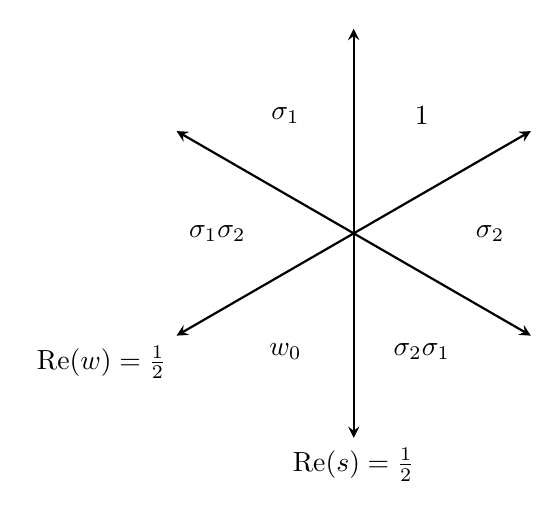
\begin{tikzpicture}[scale=3]
            \draw[thick,-stealth] (0:0) to (30:{sqrt(3)/2});
            \draw[thick,-stealth] (0:0) to (30:{-sqrt(3)/2}) node [below left] {$\Re(w) = \frac{1}{2}$};
            \draw[thick,-stealth] (0:0) to (90:{sqrt(3)/2});
            \draw[thick,-stealth] (0:0) to (90:{-sqrt(3)/2}) node [below] {$\Re(s) = \frac{1}{2}$};
            \draw[thick,-stealth] (0:0) to (150:{sqrt(3)/2});
            \draw[thick,-stealth] (0:0) to (150:{-sqrt(3)/2});

            \node at (60:{sqrt(3)/3}) {$1$};
            \node at (120:{sqrt(3)/3}) {$\s_{1}$};
            \node at (180:{sqrt(3)/3}) {$\s_{1}\s_{2}$};
            \node at (240:{sqrt(3)/3}) {$w_{0}$};
            \node at (300:{sqrt(3)/3}) {$\s_{2}\s_{1}$};
            \node at (0:{sqrt(3)/3}) {$\s_{2}$};
        \end{tikzpicture}
    \end{center}

    In the diagram, we have shifted the $(s,w)$-plane so that the origin lies at $\left(\frac{1}{2},\frac{1}{2}\right)$ and we have tiled the $(s,w)$-axes so that they are no longer perpendicular. The effect of these adjustments is that $\s_{1}$ and $\s_{2}$ act by rigid motions sending the region enclosing $1$ (corresponding to the identity) to either of the adjacent triangles. The other regions are obtained by acting by the corresponding element of $W$. The initial region $\L$ that $Z(s,w)$ is defined on is displayed in the figure below:
    
    \begin{center}
        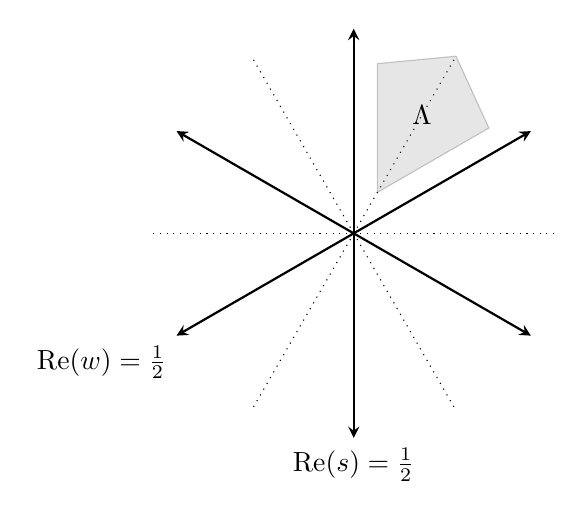
\begin{tikzpicture}[scale=3]
            \draw[dotted](0,0) to (60:{sqrt(3)/2});
            \draw[dotted](0,0) to (240:{sqrt(3)/2});
            \draw[dotted](0,0) to (180:{sqrt(3)/2});
            \draw[dotted](0,0) to (360:{sqrt(3)/2});
            \draw[dotted] (0:0) to (120:{sqrt(3)/2});
            \draw[dotted] (0:0) to (300:{sqrt(3)/2});

            \draw[thick,-stealth] (0:0) to (30:{sqrt(3)/2});
            \draw[thick,-stealth] (0:0) to (30:{-sqrt(3)/2}) node [below left] {$\Re(w) = \frac{1}{2}$};
            \draw[thick,-stealth] (0:0) to (90:{sqrt(3)/2});
            \draw[thick,-stealth] (0:0) to (90:{-sqrt(3)/2}) node [below] {$\Re(s) = \frac{1}{2}$};
            \draw[thick,-stealth] (0:0) to (150:{sqrt(3)/2});
            \draw[thick,-stealth] (0:0) to (150:{-sqrt(3)/2});


            \draw[fill=gray,opacity=0.2] (60:0.2) --+ (0,{((sqrt(5)/3)-0.2)}) -- (60:{sqrt(3)/2}) -- ($(60:0.2)+(30:{((sqrt(5)/3)-0.2)})$) -- cycle;

            \node at (60:{sqrt(3)/3}) {$\L$};
        \end{tikzpicture}
    \end{center}
    
     To meromorphically continue $Z(s,w)$ to all of the $(s,w)$-plane, we first need to show that the quadratic double Dirichlet series $Z(s,w)$ and $Z_{1,\t}(s,w)$ are locally absolutely uniformly convergent on a slightly larger region than $\L$. This will be achieved by the Phragm\'en-Lindel\"of convexity principal. Fix some small $\e > 0$. The functional equations for $L^{\ast}(s,\chi_{a_{1}d})$ and $L^{\ast}(w,\chi_{a_{2}m})$ provide the estimates
    \[
        L(-\e,\chi_{a_{1}d}) \ll |d|^{\frac{1}{2}+\e} \quad \text{and} \quad L(-\e,\chi_{a_{2}m}) \ll |m|^{\frac{1}{2}+\e},
    \]
    because $L(1+\e,\chi_{a_{1}d}) \ll 1$ and $L(1+\e,\chi_{a_{2}m}) \ll 1$. Since both of these $L$-functions have at most a simple pole at $s = 1$ and $w = 1$ respectively, the Phragm\'en-Lindel\"of convexity principal implies the weak estimates
    \[
        (s-1)L(s,\chi_{a_{1}d}) \ll |d|^{\frac{1}{2}+\e} \quad \text{and} \quad (w-1)L(w,\chi_{a_{2}m}) \ll |m|^{\frac{1}{2}+\e},
    \]
    for $\Re(s) > -\e$ and $\Re(w) > -\e$. But then from the interchange we see that $(s-1)(w-1)Z(s,w)$ and $(s-1)(w-1)Z_{1,\t}(s,w)$ are locally absolutely uniformly convergent on the region
    \[
        \L_{0} = \L \cup \left\{(s,w) \in \C^{2}:\Re(s) > 0, \Re(w) > \frac{3}{2}\right\} \cup \left\{(s,w) \in \C^{2}:\Re(s) > \frac{3}{2}, \Re(w) > 0\right\}.
    \]
    
    \begin{center}
        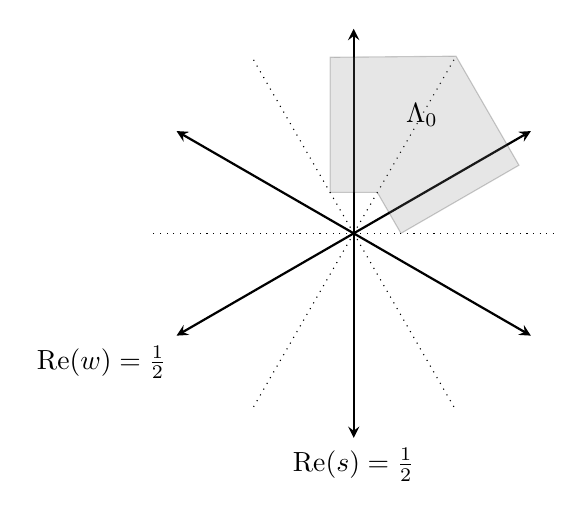
\begin{tikzpicture}[scale=3]
            \draw[dotted](0,0) to (60:{sqrt(3)/2});
            \draw[dotted](0,0) to (240:{sqrt(3)/2});
            \draw[dotted](0,0) to (180:{sqrt(3)/2});
            \draw[dotted](0,0) to (360:{sqrt(3)/2});
            \draw[dotted] (0:0) to (120:{sqrt(3)/2});
            \draw[dotted] (0:0) to (300:{sqrt(3)/2});

            \draw[thick,-stealth] (0:0) to (30:{sqrt(3)/2});
            \draw[thick,-stealth] (0:0) to (30:{-sqrt(3)/2}) node [below left] {$\Re(w) = \frac{1}{2}$};
            \draw[thick,-stealth] (0:0) to (90:{sqrt(3)/2});
            \draw[thick,-stealth] (0:0) to (90:{-sqrt(3)/2}) node [below] {$\Re(s) = \frac{1}{2}$};
            \draw[thick,-stealth] (0:0) to (150:{sqrt(3)/2});
            \draw[thick,-stealth] (0:0) to (150:{-sqrt(3)/2});

            \draw[fill=gray,opacity=0.2] (0:0.2) --+ (30:{cos(30)*((sqrt(3)/2)-0.2)}) -- (60:{sqrt(3)/2}) -- ($(120:0.2)+(0,{sqrt(5)/3-sin(120)*0.2})$) -- (120:0.2) -- (60:0.2) -- cycle;

            \node at (60:{sqrt(3)/3}) {$\L_{0}$};
        \end{tikzpicture}
    \end{center}
    
    In particular, $Z(s,w)$ and $Z_{1,\t}(s,w)$ are meromorphic on this region with at most polar lines at $s = 1$ and $w = 1$. The advantage of the region $\L_{0}$ over the initial region $\L$ is that $\L_{0}$ intersects the hyperplanes $s = \frac{1}{2}$ and $w = \frac{1}{2}$ so that the union of the reflections $w\L_{0}$ for $w \in W$ is connected. This guarantees that the functional equations imply meromorphic continuation since adjacent reflections of $\L_{0}$ overlap on open sets. The idea now is to reflect $\L_{0}$ via the functional equations and then apply a theorem of Bochner. To state this theorem we need a small definition. We say that a domain $\W \subset \C^{n}$ is a \textbf{tube domain} if there is an open set $\w \subset \R^{n}$ such that
    \[
        \W = \{(s_{1},\ldots,s_{n}) \in \C^{n}:\Re((s_{1},\ldots,s_{n})) \in \w\}.
    \]
    Tube domains are generalizations of vertical strips in the complex plane. Now we can state the theorem of Bochner (see \cite{hormander2000introduction} for a proof):

    \begin{theorem}[Bochner's continuation theorem]
        If $\W$ is a connected tube domain, then any holomorphic function on $\W$ can be extended to a holomorphic function on the convex hull $\what{\W}$.
    \end{theorem}

    By clearing polar divisors, Bochner's continuation theorem implies that any meromorphic function on a connected tube domain possessing a finite amount of hyperplane polar divisors can be extended to a meromorphic function on the convex hull. This is exactly the situation for $Z(s,w)$. Indeed, it is clear that a union of tube domains is a tube domain and so, in particular, $\L_{0}$ is a tube domain. But on $\L_{0}$ there are a most polar lines at $s = 1$ and $w = 1$. Reflecting these hyperplanes via $W$ we obtain the finite set of possible polar divisors:
    \[
        \left\{s = 1, w = 1, s = 0, w = 0, s+w = \frac{1}{2}, s+w = \frac{3}{2}\right\}.
    \]
    Therefore we are reduced to extending $Z(s,w)$ meromorphically. By applying the functional equations corresponding to $\s_{1}$, $\s_{2}$, and $\s_{1}\s_{2}$, $Z(s,w)$ admits meromorphic continuation to the region
    \[
        \L_{12} = \L_{0} \cup \s_{1}\L_{0} \cup \s_{2}\L_{0} \cup \s_{1}\s_{2}\L_{0}.
    \]

    \begin{center}
        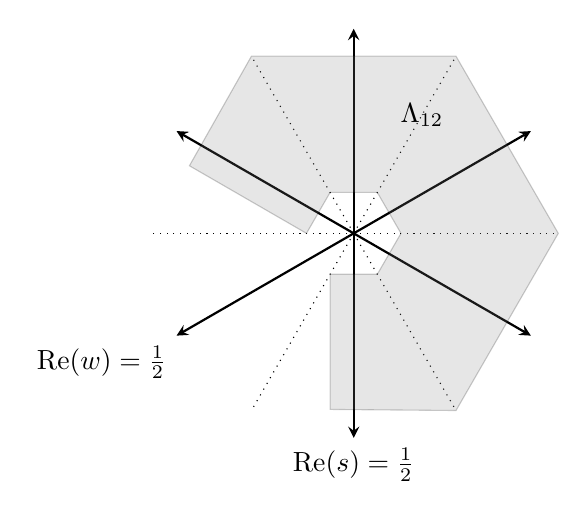
\begin{tikzpicture}[scale=3]
            \draw[dotted](0,0) to (60:{sqrt(3)/2});
            \draw[dotted](0,0) to (240:{sqrt(3)/2});
            \draw[dotted](0,0) to (180:{sqrt(3)/2});
            \draw[dotted](0,0) to (360:{sqrt(3)/2});
            \draw[dotted] (0:0) to (120:{sqrt(3)/2});
            \draw[dotted] (0:0) to (300:{sqrt(3)/2});

            \draw[thick,-stealth] (0:0) to (30:{sqrt(3)/2});
            \draw[thick,-stealth] (0:0) to (30:{-sqrt(3)/2}) node [below left] {$\Re(w) = \frac{1}{2}$};
            \draw[thick,-stealth] (0:0) to (90:{sqrt(3)/2});
            \draw[thick,-stealth] (0:0) to (90:{-sqrt(3)/2}) node [below] {$\Re(s) = \frac{1}{2}$};
            \draw[thick,-stealth] (0:0) to (150:{sqrt(3)/2});
            \draw[thick,-stealth] (0:0) to (150:{-sqrt(3)/2});

            \draw[fill=gray,opacity=0.2] (240:0.2) --+ (0,{-((sqrt(5)/3)+sin(240)*0.2)}) -- (300:{sqrt(3)/2}) -- (0:{sqrt(3)/2}) -- (60:{sqrt(3)/2}) -- (120:{sqrt(3)/2}) -- ($(180:0.2)+(150:{((sqrt(5)/3)+cos(150)*0.2)})$) -- (180:0.2) -- (120:0.2) -- (60:0.2) -- (0:0.2)-- (300:0.2) -- cycle;

            \node at (60:{sqrt(3)/3}) {$\L_{12}$};
        \end{tikzpicture}
    \end{center}

    Because the functional equations for $Z(s,w)$ involve both $Z(s,w)$ and $Z_{1,\t}(s,w)$, it was necessary to show that both of these quadratic double Dirichlet series were locally absolutely uniformly convergent on $\L_{0}$ before we applied the functional equation. Now $\L_{12}$ is a connected tube domain whose convex hull is $\C^{2}$. So by applying Bochner's continuation theorem (or rather our comment for meromorphic functions) we see that $Z(s,w)$ admits meromorphic continuation to the $(s,w)$-plane with at most a finite set of polar divisors. This method is better than repeatedly applying the functional equations corresponding to every $w \in W$. Indeed, if we did we would obtain meromorphic continuation to the region
    \[
        \L_{W} = \bigcup_{w \in W} w\L_{0}.
    \]

    \begin{center}
        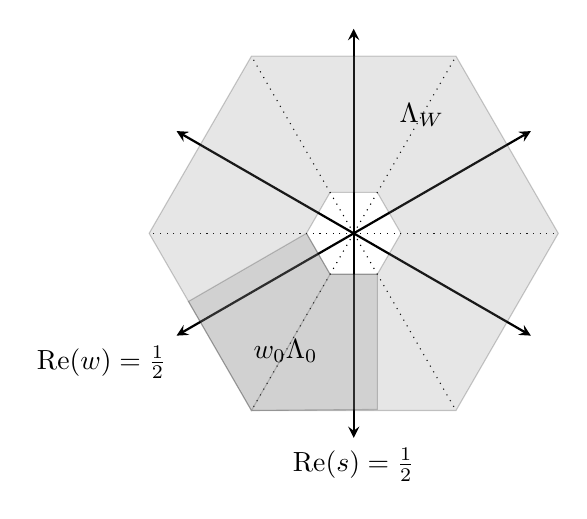
\begin{tikzpicture}[scale=3]
            \draw[dotted](0,0) to (60:{sqrt(3)/2});
            \draw[dotted](0,0) to (240:{sqrt(3)/2});
            \draw[dotted](0,0) to (180:{sqrt(3)/2});
            \draw[dotted](0,0) to (360:{sqrt(3)/2});
            \draw[dotted] (0:0) to (120:{sqrt(3)/2});
            \draw[dotted] (0:0) to (300:{sqrt(3)/2});

            \draw[thick,-stealth] (0:0) to (30:{sqrt(3)/2});
            \draw[thick,-stealth] (0:0) to (30:{-sqrt(3)/2}) node [below left] {$\Re(w) = \frac{1}{2}$};
            \draw[thick,-stealth] (0:0) to (90:{sqrt(3)/2});
            \draw[thick,-stealth] (0:0) to (90:{-sqrt(3)/2}) node [below] {$\Re(s) = \frac{1}{2}$};
            \draw[thick,-stealth] (0:0) to (150:{sqrt(3)/2});
            \draw[thick,-stealth] (0:0) to (150:{-sqrt(3)/2});
        
            \draw[fill=gray,opacity=0.2] (240:{sqrt(3)/2}) -- (300:{sqrt(3)/2}) -- (0:{sqrt(3)/2}) -- (60:{sqrt(3)/2}) -- (120:{sqrt(3)/2}) -- (180:{sqrt(3)/2}) -- (240:{sqrt(3)/2}) -- (240:0.2) -- (180:0.2) -- (120:0.2) -- (60:0.2) -- (0:0.2) -- (300:0.2) -- (240:0.2) -- cycle;

            \draw[fill=gray,opacity=0.2] (180:0.2) --+ (210:{-cos(210)*((sqrt(3)/2)-0.2)}) -- (240:{sqrt(3)/2}) -- ($(300:0.2)+(0,{-((sqrt(5)/3)+sin(300)*0.2)})$) -- (300:0.2) -- (240:0.2) -- cycle; 

            \node at (60:{sqrt(3)/3}) {$\L_{W}$};
            \node at (240:{sqrt(3)/3}) {$w_{0}\L_{0}$};
        \end{tikzpicture}
    \end{center}
    
    There are two issues here. The first is that $Z(s,w)$ has two meromorphic continuations to the region $w_{0}\L_{0}$ given by the functional equations corresponding to $w_{0} = \s_{1}\s_{2}\s_{1}$ and $w_{0} = \s_{2}\s_{1}\s_{2}$ and we would need to show that these agree. The second is that we have not obtained meromorphic continuation to $\C^{2}-\L_{W}$ which is a compact hexagon about the origin. By using Bochner's theorem after meromorphically continuing to $\L_{12}$, we have avoided these issues and as a consequence shown that the meromorphic continuations given by $w_{0} = \s_{1}\s_{2}\s_{1}$ and $w_{0} = \s_{2}\s_{1}\s_{2}$ agree.
\section{Poles \& Residues}
    We will inspect the polar divisors of $Z(s,w)$ more carefully. It turns out that the set of polar divisors is smaller than
    \[
        \left\{s = 1, w = 1, s = 0, w = 0, s+w = \frac{1}{2}, s+w = \frac{3}{2}\right\}.
    \]
    Indeed, there are no poles on the hyperplanes $s = 0$, $w = 0$, and $s+w = \frac{3}{2}$. To see this, first note that by our earlier application of the Phragm\'en-Lindel\"of convexity principal we actually obtained continuation to an open set containing $\L_{0}$ (because our estimates held for $\Re(s) > -\e$ and $\Re(w) > -\e$). We did not need this larger region for the meromorphic continuation but we do need it to study the poles. Now consider the possible polar divisor $s = 0$. We know $(s-1)(w-1)Z(s,w)$ and $(s-1)(w-1)Z_{1,\t}(s,w)$ are holomorphic on an open set containing $\L_{0}$ which contains half of the hyperplane defined by $s = 0$ outside of the hexagon $\C^{2}-\L_{W}$. As $(s-1)(w-1)$ is holomorphic on this region it follows that $Z(s,w)$ and $Z_{1,\t}(s,w)$ do not have a polar divisor at $s = 0$ on an open set containing $\L_{0}$. Now note that an open set containing $\s_{1}\s_{2}\L_{0}$ contains the other half of the hyperplane defined by $s = 0$ outside of the hexagon $\C^{2}-\L_{W}$. Upon applying the functional equation corresponding to $\s_{1}\s_{2}$, \cref{thm:double_Dirichlet_series_functional_equation} implies that the gamma factors in the corresponding functional equation have a simple pole when $s+w = \frac{3}{2}$ (the gamma factors in the functional equation for $\s_{1}$ have a simple pole at $s = 1$ and $s-1 \to s+w-\frac{3}{2}$ under $\s_{2}$). Therefore $Z(s,w)$ and $Z_{1,\t}(s,w)$ do not have polar divisors at $s = 0$ on an open set containing $\s_{1}\s_{2}\L_{0}$ away from $s+w = \frac{3}{2}$. In particular, $Z(s,w)$ does not have a polar divisor at $s = 0$ on $\L_{W}$ and away from the other polar divisors. By Bochner's continuation theorem (after clearing all of the other possible polar divisors), we see that $Z(s,w)$ does not have a polar divisors at $s = 0$ on all of $\C^{2}$ and away from the other polar divisors. An identical argument holds for the case $w = 0$ with the regions $\L_{0}$ and $\s_{2}\s_{1}\L_{0}$. For the polar divisor $s+w = \frac{1}{2}$, we argue in the same way with the regions $\s_{2}\s_{1}\L_{0}$, $\s_{1}\s_{2}\L_{0}$, and $w_{0}\L_{0}$. The only difference is that for these regions the gamma factors in the corresponding functional equations are different. For the first two regions $\s_{2}\s_{1}\L_{0}$ and $\s_{1}\s_{2}\L_{0}$, the gamma factors have a simple pole when $s+w = \frac{3}{2}$. For the third region $w_{0}\L_{0}$, the gamma factors have simple poles at $s = 1$ and $w = 1$ which is seen by using both representations $w_{0} = \s_{1}\s_{2}\s_{1}$ and $w_{0} = \s_{2}\s_{1}\s_{2}$. So in conclusion, there are no poles on the hyperplanes $s = 0$, $w = 0$, and $s+w = \frac{1}{2}$ and away from the other polar divisors. As for the hyperplanes $s = 1$, $w = 1$, and $s+w = \frac{3}{2}$, there are clearly genuine poles for $s = 1$ and $w = 1$ coming from $L(s,\chi_{d_{0}})$ and $L(w,\chi_{m_{0}})$ when $d$ and $m$ are perfect squares (so that $d_{0} = m_{0} = 1$). For $s+w = \frac{3}{2}$, we have a pole coming from the gamma factors corresponding to the functional equations for $\s_{2}\s_{1}$ and $\s_{1}\s_{2}$. We collect all of our work as a theorem:

    \begin{theorem}
        $Z(s,w)$ admits meromorphic continuation to $\C^{2}$ with polar divisors $s = 1$, $w = 1$, and $s+w = \frac{3}{2}$.
    \end{theorem}

    We can now look at the residues of $Z(s,w)$ at these poles. Since all of the poles are obtained from each other by applying the functional equations of $Z(s,w)$, we begin by looking at the pole when $w = 1$. To compute the residue we use the representation
    \[
        Z(s,w) = \sum_{\text{$m$ monic}}\frac{L(w,\chi_{m_{0}})Q_{m_{0}m_{1}^{2}}(w)}{|m|^{s}},
    \]
    coming from the interchange. For a fixed $m$, the numerator $L(w,\chi_{m_{0}})Q_{m_{0}m_{1}^{2}}(w)$ in the summand has a pole at $w = 1$ if and only if $m_{0}$ is a perfect square, that is $m_{0} = 1$, or equivalently $m = m_{1}^{2}$ itself is a perfect square. In this case, $L(w,\chi_{m_{0}}) = \z(w)$ so that
    \[
        \Res_{w = 1}L(w,\chi_{m_{0}})Q_{m_{0}m_{1}^{2}}(w) = \frac{1}{\log(q)}Q_{m_{1}^{2}}(1).
    \]
    But from \cref{lem:prime_correction_even,thm:correction_polynomial_Euler_product} we see that $Q_{m_{1}^{2}}(1) = 1$, and so
    \[
        \Res_{w = 1}Z(s,w) = \frac{1}{\log(q)}\sum_{\text{$m$ monic perfect square}}\frac{Q_{m_{1}^{2}}(1)}{|m|^{s}} = \frac{1}{\log(q)}\sum_{\text{$m$ monic}}\frac{1}{|m|^{2s}} = \frac{1}{\log(q)}\z(2s).
    \]
    Notice that this expression has a simple pole at $s = \frac{1}{2}$ which is exactly when the polar lines $w = 1$ and $s+w = \frac{3}{2}$ intersect. The residue of $Z(s,w)$ at $s = 1$ is computed in an analogous way. Indeed, by applying the interchange, the exact same argument holds with the roles of $s$ and $w$ interchanged so that
    \[
        \Res_{s = 1}Z(s,w) = \frac{1}{\log(q)}\z(2w).
    \]
    Again, this expression has a simple pole at $w = \frac{1}{2}$ which is when the polar lines $s = 1$ and $s+w = \frac{3}{2}$ intersect. The other residues at the simple poles can be computed by applying the functional equations for $Z(s,w)$ and using the residues at $s = 1$ and $w = 1$. Now consider the point where the polar lines $w = 1$ and $s+w = \frac{3}{2}$ intersect. Setting $s = \frac{1}{2}$, we see that $Z\left(\frac{1}{2},w\right)$ has a pole at $w= 1$ and we would like to understand this pole better. To accomplish this, the Mittag-Leffler theorem applied to $Z(s,w)$ (in $w$) implies that
    \[
        Z(s,w) = \frac{R_{1}(s)}{w-1}+\frac{R_{2}(s)}{s+w-\frac{3}{2}}+V(s,w),
    \]
    in some neighborhood of $\left(\frac{1}{2},1\right)$, where $V(s,w)$ is holomorphic, and we have set
    \[
        R_{1}(s) = \Res_{w = 1}Z(s,w) \quad \text{and} \quad R_{2}(s) = \Res_{w = \frac{3}{2}-s}Z(s,w).
    \]
    From our residue computations, $R_{1}(s) = \frac{1}{\log(q)}\z(2s)$ which implies that it has a simple pole at $s = \frac{1}{2}$. The residue is given by $A = \frac{1}{2\log(q)}$. On the other hand, $Z\left(\frac{1}{2},w\right)$ is holomorphic for $\Re(w) > 1$. These two facts together imply that $R_{2}(s)$ must have a simple pole at $s = \frac{1}{2}$ which cancels the simple pole coming from $R_{1}(s)$. So by Mittag-Leffler again, we may write
    \[
        R_{1}(s) = \frac{A}{s-\frac{1}{2}}+R_{3}(s) \quad \text{and} \quad R_{2}(s) = -\frac{A}{s-\frac{1}{2}}+R_{4}(s),
    \]
    in a neighborhood of $s = \frac{1}{2}$ and where $R_{3}(s)$ and $R_{4}(s)$ are holomorphic. Then
    \begin{align*}
        Z(s,w) &= \frac{R_{1}(s)}{w-1}+\frac{R_{2}(s)}{s+w-\frac{3}{2}}+V(s,w) \\ 
        &= \frac{A}{(w-1)\left(s-\frac{1}{2}\right)}+\frac{R_{3}(s)}{w-1}-\frac{A}{\left(s+w-\frac{3}{2}\right)\left(s-\frac{1}{2}\right)}+\frac{R_{4}(s)}{s+w-\frac{3}{2}}+V(s,w) \\
        &= \frac{A}{(w-1)\left(s+w-\frac{3}{2}\right)}+\frac{R_{3}(s)}{w-1}+\frac{R_{4}(s)}{s+w-\frac{3}{2}}+V(s,w).
    \end{align*}
    We can now set $s = \frac{1}{2}$ and let $B = R_{3}\left(\frac{1}{2}\right)+R_{4}\left(\frac{1}{2}\right)$ so that
    \[
        Z\left(\frac{1}{2},w\right) = \frac{A}{(w-1)^{2}}+\frac{B}{w-1}+O(1).
    \]
    It follows that $Z\left(\frac{1}{2},w\right)$ has a double pole at $w = 1$. This can be thought of as follows: the polar lines $w = 1$ and $s+w = \frac{3}{2}$ correspond to simple poles of $Z(s,w)$ except in the case when they intersect and the order of the poles combine to give $Z\left(\frac{1}{2},w\right)$ a double pole at $w = 1$. Applying the interchange, the exact same argument holds to show that $Z\left(s,\frac{1}{2}\right)$ has a double pole at $s = 1$. We collect this work as a theorem:

    \begin{theorem}\label{thm:double_poles_at_1/2}
        $Z\left(\frac{1}{2},w\right)$ and $Z\left(s,\frac{1}{2}\right)$ have double poles at $w = 1$ and $s = 1$ respectively. In particular, in neighborhoods of $w = 1$ and $s = 1$ respectively, we have
        \[
            Z\left(\frac{1}{2},w\right) = \frac{A}{(w-1)^{2}}+\frac{B}{w-1}+O(1) \quad \text{and} \quad Z\left(s,\frac{1}{2}\right) = \frac{A}{(s-1)^{2}}+\frac{B}{s-1}+O(1),
        \]
        for some constants $A$ and $B$ with $A = \frac{1}{2\log(q)}$. 
    \end{theorem}
\section{An Application}
    As an application of the usefulness of quadratic double Dirichlet series, we show that the analytic properties of $Z(s,w)$ can be used to obtain a simultaneous non-vanishing result. In particular, we show that $L\left(\frac{1}{2},\chi_{d}\right)$ is nonzero for infinitely many $d$. Since the complex analysis involved comes from standard analytic number theory techniques, strictly speaking, we only sketch the result. To being, Perron's formula implies
    \[
        \sum_{\deg(d) \le X}L\left(\frac{1}{2},\chi_{d_{0}}\right)Q_{d_{0}d_{1}^{2}}\left(\frac{1}{2}\right) = \frac{1}{2\pi i}\int_{(2)}Z\left(\frac{1}{2},w\right)X^{w}\,dw,
    \]
    for some $X > 1$. It can be shown that $Z(s,w)$ is bounded in vertical strips provided we are away from poles. It follows that \cref{thm:double_poles_at_1/2} holds in vertical strips about the lines $\Re(w) = 1$ and $\Re(s) = 1$ respectively. Therefore
    \[
        \frac{1}{2\pi i}\int_{(2)}Z\left(\frac{1}{2},w\right)X^{w}\,dw = \frac{1}{2\pi i}\int_{(2)}\left(\frac{A}{(w-1)^{2}}+\frac{B}{w-1}+O(1)\right)X^{w}\,dw.
    \]
    Shifting the line of integration to the left (say to the line $\Re(w) = -2$) and using the residue theorem, we pick up a residue from the pole at $w = 1$. The contribution from the first two terms to the residue are $AX\log(X)$ and $BX$ respectively while the third term vanishes (recall that the integrand has a factor of $X^{w}$). The remaining vertical integral is $o(X)$. Therefore
    \[
        \frac{1}{2\pi i}\int_{(2)}Z\left(\frac{1}{2},w\right)X^{w}\,dw = AX\log(X)+BX+o(X),
    \]
    it follows that
    \[
        \sum_{\deg(d) \le X}L\left(\frac{1}{2},\chi_{d_{0}}\right)Q_{d_{0}d_{1}^{2}}\left(\frac{1}{2}\right) = AX\log(X)+BX+o(X).
    \]
    But as $A = \frac{1}{2\log(q)} \neq 0$ (see \cref{thm:double_poles_at_1/2}) this means that $L\left(\frac{1}{2},\chi_{d}\right)$ must be nonzero for infinitely many $d$ (in particular for infinitely many square-free $d$). For otherwise, $\sum_{\deg(d) \le X}L\left(\frac{1}{2},\chi_{d_{0}}\right)Q_{d_{0}d_{1}^{2}}\left(\frac{1}{2}\right) = O(1)$ which gives a contradiction.
\section{\texorpdfstring{$Z(s,w)$}{Z(s,w)} as a Rational Function}
    Recall that $L(s,\chi_{d})$ is a polynomial in $q^{-s}$ of degree at most $\deg(d)-1$. A similar situation happens for the quadratic double Dirichlet series $Z(s,w)$, it will be a rational function in the variables $x = q^{-s}$ and $y = q^{-w}$. Since this property is a special case of Dirichlet series over function fields, we present the argument but suppress the more detailed computations. Before we begin, we recall some properties of Hadamard products of power series. The details can be found in \cite{stanley2023enumerative}. For any two power series
    \[
        R_{1}(x,y) = \sum_{k,l \ge 0}r_{1}(k,l)x^{k}y^{l} \quad \text{and} \quad R_{2}(x,y) = \sum_{k,l \ge 0}r_{2}(k,l)x^{k}y^{l},
    \]
    or more generally generating series, their \textbf{Hadamard product} $(R_{1} \ast R_{2})(x,y)$ is defined by
    \[
        (R_{1} \ast R_{2})(x,y) = \sum_{k,l \ge 0}r_{1}(k,l)r_{2}(k,l)x^{k}y^{l}.
    \]
    If we assume $R_{1}(x,y)$ and $R_{2}(x,y)$ are regular around the origin $x = y = 0$, then the Hadamard product can be expressed as two contour integrals around the origin:
    \[
        (R_{1} \ast R_{2})(x,y) = \frac{1}{(2\pi i)^{2}}\int_{|z| = \rho}\int_{|w| = \rho}R_{1}(z,w)R_{2}\left(\frac{x}{z},\frac{y}{w}\right)\,\frac{dz}{z}\,\frac{dw}{w},
    \]
    for sufficiently small $\rho > 0$. By the residue theorem,
    \[
        (R_{1} \ast R_{2})(x,y) = \sum_{s = s(x,y)}\Res_{s}\left(\frac{R_{1}(z,w)R_{2}\left(\frac{x}{z},\frac{y}{w}\right)}{zw}\right),
    \]
    where the sum is over all poles $s = s(x,y)$ of the integrand such that $\lim_{x,y \to 0}s(x,y) = 0$. This formula can be used to compute the Hadamard product of rational functions. In the following argument where computing a Hadamard product is necessary, this method can be used.

    Now we show that $Z(s,w)$ is a rational function in $x = q^{-s}$ and $y = q^{-w}$. Throughout, we work in the region of local absolute uniform convergence for $Z(s,w)$. Consider the representation
    \[
        Z(s,w) = \sum_{\text{$d$ monic}}\frac{L(s,\chi_{d})}{|d|^{w}} = \sum_{\text{$m,d$ monic}}\frac{\chi_{d_{0}}(\what{m})H(m,d)}{|m|^{s}|d|^{w}}.
    \]
    Since $L(s,\chi_{d})$ is a polynomial in $q^{-s}$ of degree at most $\deg(d)-1$ and correction polynomials $Q_{d_{0}d_{1}^{2}}(s)$ are Dirichlet polynomials, one of the two following cases occur:
    \begin{itemize}
        \item If $d$ is a perfect square, then $L(s,\chi_{d_{0}}) = \z(s)$ and
        \[
            L(s,\chi_{d}) = \z(s)Q_{d_{1}^{2}}(s),
        \]
        where $Q_{d_{1}^{2}}(s)$ is a polynomial in $q^{-s}$ of degree $\deg(d)$.
        \item If $d$ is not a perfect square, then
        \[
            L(s,\chi_{d}) = L(s,\chi_{d_{0}})Q_{d_{0}d_{1}^{2}}(s),
        \]
        is a polynomial in $q^{-s}$ of degree at most $\deg(d)-1$.
    \end{itemize}
    So if $d$ is not a perfect square, then
    \[
        L(s,\chi_{d}) = \sum_{\deg(m) \le \deg(d)-1}\frac{\chi_{d_{0}}(\what{m})H(m,d)}{|m|^{s}},
    \]
    which is to say that
    \[
        \sum_{\deg(m) = k}\chi_{d_{0}}(\what{m})H(m,d) = 0,
    \]
    for every $k \ge \deg(d)$ provided $d$ is not a perfect square. To exploit this fact, we will decompose $Z(s,w)$ according to whether $\deg(d) \ge \deg(m)$ or $\deg(d) \le \deg(m)$. So we write
    \[
        Z(s,w) = Z_{0}(s,w)+Z_{0}(w,s)-Z_{1}(s,w),
    \]
    where
    \[
        Z_{0}(s,w) = \sum_{0 \le l \le k}\frac{1}{q^{ls}q^{kw}}\sum_{\substack{\text{$m,d$ monic} \\ \deg(m) = k \\ \deg(d) = l}}\chi_{d_{0}}(\what{m})H(m,d) \quad \text{and} \quad Z_{1}(s,w) = \sum_{k \ge 0}\frac{1}{q^{ks}q^{kw}}\sum_{\substack{\text{$m,d$ monic} \\ \deg(m) = k \\ \deg(d) = k}}\chi_{d_{0}}(\what{m})H(m,d).
    \]
    We will now show that $Z_{0}(s,w)$ and $Z_{1}(s,w)$ are rational functions in $q^{-s}$ and $q^{-w}$ via a convolution procedure. For $Z_{0}(s,w)$, our remarks about $L(s,\chi_{d})$ imply the term in the inner sum of $Z_{0}(s,w)$ vanishes unless $d$ is a perfect square and in this case $\chi_{d_{0}}(\what{m}) = 1$. Therefore
    \[
        Z_{0}(s,w) = \sum_{0 \le l \le k}\frac{1}{q^{ls}q^{kw}}\sum_{\substack{\text{$m,d$ monic} \\ \text{$d$ a perfect square} \\ \deg(m) = l \\ \deg(d) = k}}H(m,d).
    \]
    Now consider
    \[
        Y(s,w) = \sum_{\substack{\text{$m,d$ monic} \\ \text{$d$ monic perfect square}}}\frac{H(m,d)}{|m|^{s}|d|^{w}} \quad \text{and} \quad K_{0}(s,w) = \sum_{0 \le l \le k}\frac{1}{q^{ls}q^{kw}}.
    \]
    We can express both of these as rational functions in $q^{-s}$ and $q^{-w}$. Indeed, for $Y(s,w)$, \cref{prop:multiplicativity_of_weighting_coefficients}  we that $Y(s,w)$ possesses a Euler product. Using \cref{cor:evaulation_of_weighting_coefficients_at_primes}, we compute
    \[
        Y(s,w) = \frac{1-q^{1-s-2w}}{(1-q^{1-2w})(1-q^{1-s})(1-q^{2-2s-2w})},
    \]
    which can also be seen by comparing coefficients of the power series expansion of the right-hand side. $K_{0}(s,w)$ is even easier because it is a geometric series:
    \[
        K_{0}(s,w) = \sum_{0 \le l \le k}\frac{1}{q^{ls}q^{kw}} = \frac{1}{(1-q^{-s})(1-q^{-s-w})}.
    \]
    Then $Z_{0}(s,w)$ is expressed as a Hadamard product of power series in $q^{-s}$ and $q^{-w}$:
    \[
        Z_{0}(s,w) = Y(s,w) \ast K_{0}(s,w).
    \]
    Then using the contour integral representation of the Hadamard product, we compute
    \[
        Z_{0}(s,w) = \frac{1}{(1-q^{1-s})(1-q^{3-2s-2w})}.
    \]
    For $Z_{1}(s,w)$, our remarks about $L(s,\chi_{d})$ similarly imply
    \[
        Z_{1}(s,w) = \sum_{k \ge 0}\frac{1}{q^{ks}q^{kw}}\sum_{\substack{\text{$m,d$ monic} \\ \text{$d$ a perfect square} \\ \deg(m) = k \\ \deg(d) = k}}H(m,d).
    \]
    But then we may repeat the same argument as for $Z_{0}(s,w)$ with
    \[
        Y(s,w) = \sum_{\substack{\text{$m,d$ monic} \\ \text{$d$ monic perfect square}}}\frac{H(m,d)}{|m|^{s}|d|^{w}} \quad \text{and} \quad K_{1}(s,w) = \sum_{k \ge 0}\frac{1}{q^{ks}q^{kw}},
    \]
    and arrive at
    \[
        Z_{1}(s,w) = \frac{1}{(1-q^{3-2s-2w})}.
    \]
    Combining these representations for $Z_{0}(s,w)$ and $Z_{1}(s,w)$ with our decomposition of $Z(s,w)$ yields
    \[
        Z(s,w) = \frac{1-q^{2-s-w}}{(1-q^{1-s})(1-q^{1-w})(1-q^{3-2s-2w})}.
    \]
    Setting $x = q^{-s}$ and $y = q^{-w}$ gives
    \[
        Z(x,y) = \frac{1-q^{2}xy}{(1-qx)(1-qy)(1-q^{3}x^{2}y^{2})},
    \]
    which is a rational function in $x$ and $y$.

    \begin{remark}
        Some authors, especially those using the Chinta-Gunnells construction of building multiple Dirichlet series, prefer the $W$-invariant point to be at the origin. For this, we make the change of variables $\left(s+\frac{1}{2},w+\frac{1}{2}\right) \to (s,w)$ which gives
        \[
            Z(s,w) = \frac{1-q^{1-s-w}}{(1-q^{\frac{1}{2}-s})(1-q^{\frac{1}{2}-w})(2-q^{3-2s-2w})},
        \]
         and upon setting $x = q^{-s}$ and $y = q^{-w}$, we have
        \[
            Z(x,y) = \frac{1-qxy}{(1-q^{\frac{1}{2}}x)(1-q^{\frac{1}{2}}y)(1-q^{2}x^{2}y^{2})}.
        \]
    \end{remark}

\appendix
\section{Generating Functions for the Weighting Coefficients}
    In this appendix we discuss properties of the generating function for the weighting coefficients $H(P^{k},P^{l})$ for a fixed irreducible $P$. This generating function has the same functional equations as $Z(s,w)$, and it is this property that motivated the Chinta-Gunnells construction. For a fixed irreducible $P$, define
    \[
        H(s,w) = \sum_{k,l \ge 0}\frac{H(P^{k},P^{l})}{|P|^{ks}|P|^{lw}}.
    \]
    From \cref{cor:evaulation_of_weighting_coefficients_at_primes}, $H(x,y)$ is locally absolutely uniformly convergent provided $\Re(s) > 1$ and $\Re(w) > 1$. To obtain the generating function, we set $x = |P|^{-s}$ and $y = |P|^{-w}$ so that
    \[
        H(x,y) = \sum_{k,l \ge 0}H(P^{k},P^{l})x^{k}y^{l},
    \]
    where this series is locally absolutely uniformly convergent for $|x| < |P|^{-1}$ and $|y| < |P|^{-1}$. Now let $x = |P|^{-s}$ in $Q_{P^{2\a+1}}(s)$ and $Q_{P^{2\b}}(s)$ and denote the resulting functions as $Q_{P^{2\a+1}}(x)$ and $Q_{P^{2\b}}(x)$. Then by \cref{lem:prime_correction_odd,lem:prime_correction_even,cor:evaulation_of_weighting_coefficients_at_primes}, we have
    \[
        Q_{P^{2\a+1}}(x) = \sum_{k \ge 0}H(P^{k},P^{2\a+1})x^{k} \quad \text{and} \quad \frac{1}{1-x}Q_{P^{2\b}}(x) = \sum_{k \ge 0}H(P^{k},P^{2\b})x^{k}.
    \]
    Note that these series are over every $k \ge 0$. In the first equality we have used the fact that $H(P^{k},P^{2\a+1}) = 0$ if $k > 2\a$ and in the second equality we have used the geometric series representation $\frac{1}{1-x} = \sum_{k \ge 0}x^{k}$. Upon taking the subseries of $H(x,y)$ with $l$ fixed, namely $\sum_{k \ge 0}H(P^{k},P^{l})x^{k}$, we obtain
    \[
        \sum_{k \ge 0}H(P^{k},P^{l})x^{k} = \begin{cases} Q_{P^{l}}(x) & \text{if $l$ is odd}, \\ \frac{1}{1-x}Q_{P^{l}}(x) & \text{if $l$ is even}. \end{cases}
    \]
    The functional equation \cref{thm:functional_equation_correction_polynomials} will induce functional equations for $Q_{P^{l}}(x)$ ($l$ is even or odd) and this will further induce functional equations for $H(x,y)$. To see this, if $s \to 1-s$ then $x \to \frac{1}{|P|x}$ and so \cref{thm:functional_equation_correction_polynomials} implies the functional equation
    \[
        Q_{P^{2l+i}}(x) = |P|^{l}x^{2l}Q_{P^{2l+i}}\left(\frac{1}{|P|x}\right),
    \]
    for $i = 0,1$. Now let
    \[
        H_{y}^{\pm}(x,y) = \frac{H(x,y)\pm H(x,-y)}{2}.
    \]
    That is, $H_{y}^{\pm}(x,y)$ is the subseries of $H(x,y)$ consisting of those terms with $l$ even or odd respectively. Equivalently,
    \[
        H_{y}^{+}(x,y) = \sum_{l \ge 0}Q_{P^{2l}}(x)y^{2l} \quad \text{and} \quad H_{y}^{-}(x,y) = \sum_{l \ge 0}Q_{P^{2l+1}}(x)y^{2l+1}.
    \]
    Applying the functional equation for $Q_{P^{2l+i}}(x)$ to $H_{y}^{+}(x,y)$ and $H_{y}^{-}(x,y)$, we obtain functional equations
    \[
        (1-x)H_{y}^{+}(x,y) = \left(1-\frac{1}{|P|x}\right)H_{y}^{+}\left(\frac{1}{|P|x},\sqrt{|P|}xy\right) \quad \text{and} \quad H_{y}^{-}(x,y) = \frac{1}{\sqrt{|P|x}}H_{y}^{-}\left(\frac{1}{|P|x},\sqrt{|P|}xy\right).
    \]
    Similarly, let
    \[
        H_{x}^{\pm}(x,y) = \frac{H(x,y)\pm H(-x,y)}{2}.
    \]
    That is, $H_{x}^{\pm}(x,y)$ is the subseries of $H(x,y)$ consisting of those terms with $k$ even or odd respectively. Equivalently,
    \[
        H_{x}^{+}(x,y) = \sum_{k \ge 0}Q_{P^{2k}}(x)x^{2k} \quad \text{and} \quad H_{x}^{-}(x,y) = \sum_{k \ge 0}Q_{P^{2k+1}}(x)x^{2k+1}.
    \]
    Then we have functional equations
    \[
        (1-y)H_{x}^{+}(x,y) = \left(1-\frac{1}{|P|y}\right)H_{x}^{+}\left(\sqrt{|P|}xy,\frac{1}{|P|y}\right) \quad \text{and} \quad H_{x}^{-}(x,y) = \frac{1}{\sqrt{|P|y}}H_{x}^{-}\left(\sqrt{|P|}xy,\frac{1}{|P|y}\right).
    \]
    We can state these four functional equations in a more compact form. For $f \in \C(x,y)$, let $f_{y}^{\pm}$ and $f_{x}^{\pm}$ be the even and odd parts of $f$ with respect to $y$ and $x$ respectively. As $H(x,y) = H_{y}^{+}(x,y)+H_{y}^{-}(x,y)$ and $H(x,y) = H_{x}^{+}(x,y)+H_{x}^{-}(x,y)$, these pairs of functional equations are equivalent to $H(x,y)$ being invariant under the actions $|^{\mathrm{CG}}\s_{1}$ and $|^{\mathrm{CG}}\s_{2}$ on $\C(x,y)$ defined by
    \[
        f(x,y)|^{\mathrm{CG}}\s_{1} = -\frac{1-|P|x}{|P|x(1-x)}f_{y}^{+}\left(\frac{1}{|P|x},\sqrt{|P|}xy\right)+\frac{1}{\sqrt{|P|}x}f_{y}^{-}\left(\frac{1}{|P|x},\sqrt{|P|}xy\right),
    \]
    and
    \[
        f(x,y)|^{\mathrm{CG}}\s_{2} = -\frac{1-|P|y}{|P|y(1-y)}f_{x}^{+}\left(\sqrt{|P|}xy,\frac{1}{|P|y}\right)+\frac{1}{\sqrt{|P|}y}f_{x}^{-}\left(\sqrt{|P|}xy,\frac{1}{|P|x}\right).
    \]
    These two actions are precisely the Chinta-Gunnels actions corresponding to the simple reflections $\s_{1}$ and $\s_{2}$. It can be verified directly that these actions extend to an action of $W$ on $\C(x,y)$. Therefore $H(x,y)$ has the same group of functional equations as $Z(s,w)$.

    \bibliographystyle{plain}
    \bibliography{Twiss2024quadratic(I)}

\end{document}